\documentclass[12pt]{mitthesis} 

\usepackage{lgrind, braket, amsmath,
  amssymb, bbm, booktabs, subfig, color} 
\usepackage[pdftex]{graphicx}
\usepackage[version=3]{mhchem}

\newcommand{\TODO} [1]{\textcolor{magenta}{\textbf{TODO:} #1}}
\newcommand{\POINT}[1]{\textcolor{magenta}{#1}}

\hyphenation{acetylene}
\hyphenation{Hamiltonian}

\begin{document}

\tableofcontents
\clearpage

\subsubsection*{NOTES}

\clearpage

\chapter{SEELEM/LIF spectroscopy of 
%\emph{ungerade}  vibrational levels of 
  acetylene $S_1$: 
%contrasting singlet-triplet dynamical behavior
spectral patterns of mediated spin-orbit coupling
}

\section{Introduction}

\POINT{Show the vibrational modes of \emph{trans} acetylene and their
  symmetries.  Explain selection rules for transitions from the ground
  state.  (See p.33 of1/2007--3/2007 notebook.)}

\POINT{Summarize current understanding of spin-orbit coupling in
  acetylene.  Refer to chapter 1?  Coupling between $S_1$ and
  $T_{1,2}$ is mediated by $T_3$.}

\POINT{Make the case for studying non-symmetric bending motions in
  acetylene.  The $T_3$ state is bent out-of-plane.  However, several
  observations have been made that mode 6 is more active in promoting
  ISC.  How does this jive with our distant doorway theory?}

\POINT{The out-of-plane bending mode in acetylene $S_1$ is strongly
  mixed with the antisymmetric in-plane bend, so we must study them in
  tandem.}

\POINT{Recent breakthrough in our understanding of these bending
  polyads.  Energies and eigenvectors predicted by AHS and Merer.
  Overlap with $T_3$ levels predicted by Bryan and Ryan.  (See p.40 of
  1/2007--3/2007 notebook.)}

\POINT{Make the case for studying the role of $\nu_3$ in ISC.  Cite
  trends observed on ZAC papers.  We consider three bands in roughly
  the same energy region.}

\TODO{Adapt the following from the article.}  Surface Electron
Ejection by Laser-Excited Metastables1-3 (SEELEM) and LIF spectroscopy
are complementary tools that have been used to gain insight into
singlet $\sim$ triplet interactions in the Ã1Au X 1Σg+ (S1-S0) electronic
spectrum of acetylene, C2H2.3-6 LIF detection is limited to
short-lived ($\tau$radiative < 10 $\mu$s), strongly fluorescing singlet
states, while SEELEM detection is sensitive only to long-lived ($\tau$>
300 $\mu$s) states with vertical electronic excitation above a threshold
energy set by the work function of the metal used as the SEELEM
detector surface. Therefore, SEELEM and LIF detection channels observe
mutually exclusive sets of eigenstates that arise from spin-orbit
mixed S1,T3,2,1 zero-order basis states.  A comparison of
simultaneously recorded SEELEM and LIF spectra reveals features of
electronic structure and photochemical pathways that are invisible via
traditional, single-channel spectroscopic probes such as LIF alone,
REMPI, phosphorescence, phosphor surface, etc.7-8 The information
gained from comparison of acetylene SEELEM / LIF spectra can yield a
mechanistic description of singlet $\sim$ triplet interaction, and holds
promise for describing the structure and dynamics of other small
polyatomic species.9,10 Dupré et al.11,12 have determined that the
singlet $\sim$ triplet dynamics of acetylene near the region of the Ã1Au
state are governed by a doorway mediated mechanism,3-6,13 where
particular vibrational levels of the $T_3$ state provide a doorway for
intersystem crossing between the initially excited $S_1$ bright state and
the dense manifold of dark T1,2 states.

The Ã1Au - X 1Σg+ electronic band system of acetylene is one of the
most thoroughly examined electronic transitions of any polyatomic
molecule.14-19 Despite numerous investigations, only a partial picture
of Ã1Au state vibrational structure and interactions has been
developed. Several researchers have used double resonance techniques
to detect and analyze transitions to the ν4 and ν6 fundamentals,
overtones, and combination bands in the Ã1Au state. Utz et. al. were
the first to unambiguously assign electronic transitions to the Ã1Au
state ν4 (torsion) and ν6 (antisymmetric in-plane bend) vibrational
fundamentals using pulsed laser double resonance in a room temperature
cell.20 They observed strong a- and b-axis Coriolis interactions
between the two nearly degenerate bending modes, and deperturbed these
interactions to obtain vibrational frequencies, Coriolis interaction
constants, and rotational constants.  That experiment is very relevant
to the work presented in this paper, since the near degeneracy of the
two vibrational fundamentals is expected to result in analogous
interactions amongst the higher lying combination and overtone levels
involving ν4 and ν6.21 Mizoguchi et. al. also observed ungerade
vibrational states via the Ã1Au - X 1Σg+ transition using IR-UV
double resonance spectroscopy.22 In particular, they excited acetylene
to its ungerade nν3’ + ν4’ and nν3’ + ν6’ (n = 2,3)
vibrational levels in the Ã1Au state via IR excitation of selected
rotational levels in the ν3” vibrational state of the X 1Σg+
electronic ground state.  They investigated the Coriolis coupling
between the combination bands involving ν4’ and ν6’, and examined
the vibrational mode dependence of the singlet $\sim$ triplet interaction
by observing splittings in the $K_a$ = 1 rotational levels of the
3ν3’ + ν6’ band. The singlet $\sim$ triplet interaction in these states
was further probed in continuing work by Yamakita and Tsuchiya,23 who
observed Zeeman quantum beats by IR-UV double resonance LIF. They
observed both rotational level splittings and Zeeman quantum beats in
the fluorescence decay of the 3ν3’ + ν6’ band.  No analogous
splitting or Zeeman quantum beats were seen in the
3ν3’ + ν4’ band. They concluded that excitation of the
out-of-plane ν4’ torsional mode suppresses the singlet $\sim$ triplet
interaction, while excitation of the in-plane antisymmetric bend, ν6’,
promotes $S_1$ $\sim$ $T_3$ interaction. From this, it was inferred that the
singlet $\sim$ triplet mixing occurs in a planar (C2h or C2v) geometry
rather than at a non- planar C2 geometry, since the
3ν3’ + ν4’ band did not exhibit any rotational line splittings or
Zeeman quantum beats.

The focus of this paper is a comparison of combination bands involving
overtones of the low- frequency bending vibrations, ν4 and ν6, of
acetylene in its Ã1Au state. In the normal mode model of acetylene
vibrational dynamics, ν4 is the only normal vibration in the Ã1Au
state that involves a motion out-of-the-plane from the planar,
trans-bent equilibrium structure of the à state, while ν6 is an
in-plane antisymmetric bend. A more sophisticated polyad model24 goes
beyond the zero-order normal mode picture by incorporating anharmonic
and vibration-rotation (including Coriolis) interactions among groups
of near degenerate states. The results of such an analysis show that
the resultant eigenstates formed from the zero-order degenerate
bending modes are profoundly mixed via strong anharmonic
(Darling-Dennison) and Coriolis interactions.25 In this case, the
simpler normal mode model is invalid, and the vibrational
wavefunctions of levels assigned to ν4 or ν6 do not resemble the
nuclear motions suggested by their labels, but are strongly mixed
superpositions of the two zero-order bending modes.  In this work, the
nominal $4^2$ and 62 spectral labels are retained, despite the fact that
the two levels are nearly 50:50 mixed.

We report on the simultaneously recorded SEELEM and LIF spectra that
sample the near- degenerate, strongly mixed $2^13^14^2$ $K_a$ = 1 and 213162
Ka = 1 vibrational levels of acetylene in its Ã1Au state. The SEELEM
spectra of these two vibrational levels are remarkably different. The
spectra provide a unique opportunity to investigate the effect of
selective vibrational excitation on the interaction between singlet
and triplet states of acetylene. One might expect the intensities in
the SEELEM spectra of the $2^13^14^2$ and $2^13^16^2$ vibrational levels to be
controlled by Franck-Condon overlap between the vibrational
wavefunctions of the interacting $S_1$ and $T_3$ electronic states. The
expectation under a normal mode model is that, since the $T_3$ electronic
state has a non-planar Cs configuration,26,27 excitation of the
in-plane ν6 mode would result in small vibrational overlap with T3,
while excitation of the out-of-plane vibration, $\nu$4, would result in
large vibrational overlap. If the normal mode model were valid,
interaction with triplet states would be promoted by excitation
of $\nu$4, resulting in large SEELEM signal, while excitation of $\nu$6
should suppress SEELEM activity. The strongly mixed nature of the Ã1Au
213142 $K_a$ = 1 and $2^13^16^2$ $K_a$ = 1 vibrational levels rules out such a
simple explanation for the contrasting SEELEM spectra observed in the
experiment. The purpose of this paper is to provide an explanation of
the difference between the SEELEM spectra involving the mixed 213142
and $2^13^16^2$ vibrational levels, and to propose a qualitative mechanism
which gives rise to the different spectral patterns. Comparison and
analysis of the SEELEM / LIF spectra will elucidate the mechanism of
the doorway S1$\sim$T3 interaction process.


\section{Patterns of spectral intensity in gated fluorescence and
  SEELEM}

\POINT{Refer to earlier chapter where SEELEM intensity distributions
  were presented for distant doorways.}  In chapter 2, we have
introduced the concept of a SEELEM intensity distribution associated
with a singlet bright state.  Here, we extend the idea of dark state
intensity distributions to fluorescence measurements by considering
the appearence of the \emph{incoherent, frequency domain} spectrum at
a time window $t+dt$ after excitation of the molecule.  The SEELEM
spectrum is shown to be an extreme, limiting case of delayed
fluorescence.  Furthermore, we demonstrate that molecular properties
such as coupling matrix element and the energy denominator for a
mediating doorway state are revealed by changes in statistical
properties of the spectrum as it changes from immediate ($t\ll\tau_s$)
LIF, into delayed LIF, and finally to SEELEM.

\TODO{Adapt following from delayedfluorescence report.}  For a pure
singlet bright state $\ket{s}$, the time-dependent fluorescence
intensity is
\begin{equation}
  I_s(t) = \frac{1}{\tau_s} \;
           \exp \left[
             -\frac{t}{ \tau_s} 
           \right],
\end{equation}
normalized such that $\int_0^{\infty} I_s(t) \, dt = 1$.

We consider the case where $\ket{s}$ is directly coupled with a set of
$N$ triplet dark states to create a set of $N$+1 mixed states
$\lbrace\ket{m}\rbrace$.  Each state $\ket{m}$ has some bright state
amplitude $a_m$.  In the case of direct or doorway-mediated coupling,
the Hamiltonian contains only one pathway from each dark state to the
bright state (see Chapter 3).  As a result, the mixing amlitudes may
be taken to be real and positive by convention.  If the lifetime of a
pure triplet dark state is much longer than $\tau_s$, the lifetime of
a mixed eigenstate $\ket{m}$ having bright state character
$\alpha_m^2$ is
\begin{equation}
  \label{eq:tau-m}
  \tau_m = \tau_s / a_m^2,
\end{equation}
and its time-dependent fluorescence intensity is
\begin{equation}
  \label{eq:int-m}
  I_m(t) = \frac{a_m^4}{\tau_s} \;
           \exp \left[
             -\frac{a_m^2 \, t}{\tau_s} 
           \right].
\end{equation}
The total integrated fluorescence intensity for a mixed state is
$\int_0^{\infty} I_m(t) \, dt = a_m^2$, relative to unit intensity for
a pure bright state.

The normalization condition for bright state character $\sum_m a_m^2 =
1$ leads to the relation
\begin{equation}
  \tau_s^{-1} = \sum_m \tau_m^{-1};
\end{equation}
in this way, $\tau_s$ can be derived from the set of mixed state
lifetimes $\lbrace \tau_m \rbrace$.

\subsection{SEELEM detection as an extreme limit of delayed fluorescence}

We examine the fluorescence intensity after a time delay $t_c$,
which we cast in units of the bright state lifetime:
\begin{equation}
  R_c = t_c / \tau_s.
\end{equation}
At a chosen $R_c$, the fluorescence intensity equation has a single
peak according to some value of bright state character.  Within the
range $0 \le a_m^2 \le 1$, the fluorescence intensity equation is at a
maximum when (Chapter 2, equation 31)
\begin{equation}
  \label{eq:am-max}
  a_m^2 = \frac{2}{R_c}.
\end{equation}

\begin{figure}
  \caption{The intensity of a mixed eigenstate at time $R_c =
    t/\tau_s$, plotted as a function of bright
    state character.}
  \label{fig:int-at-rc}
  \centering
  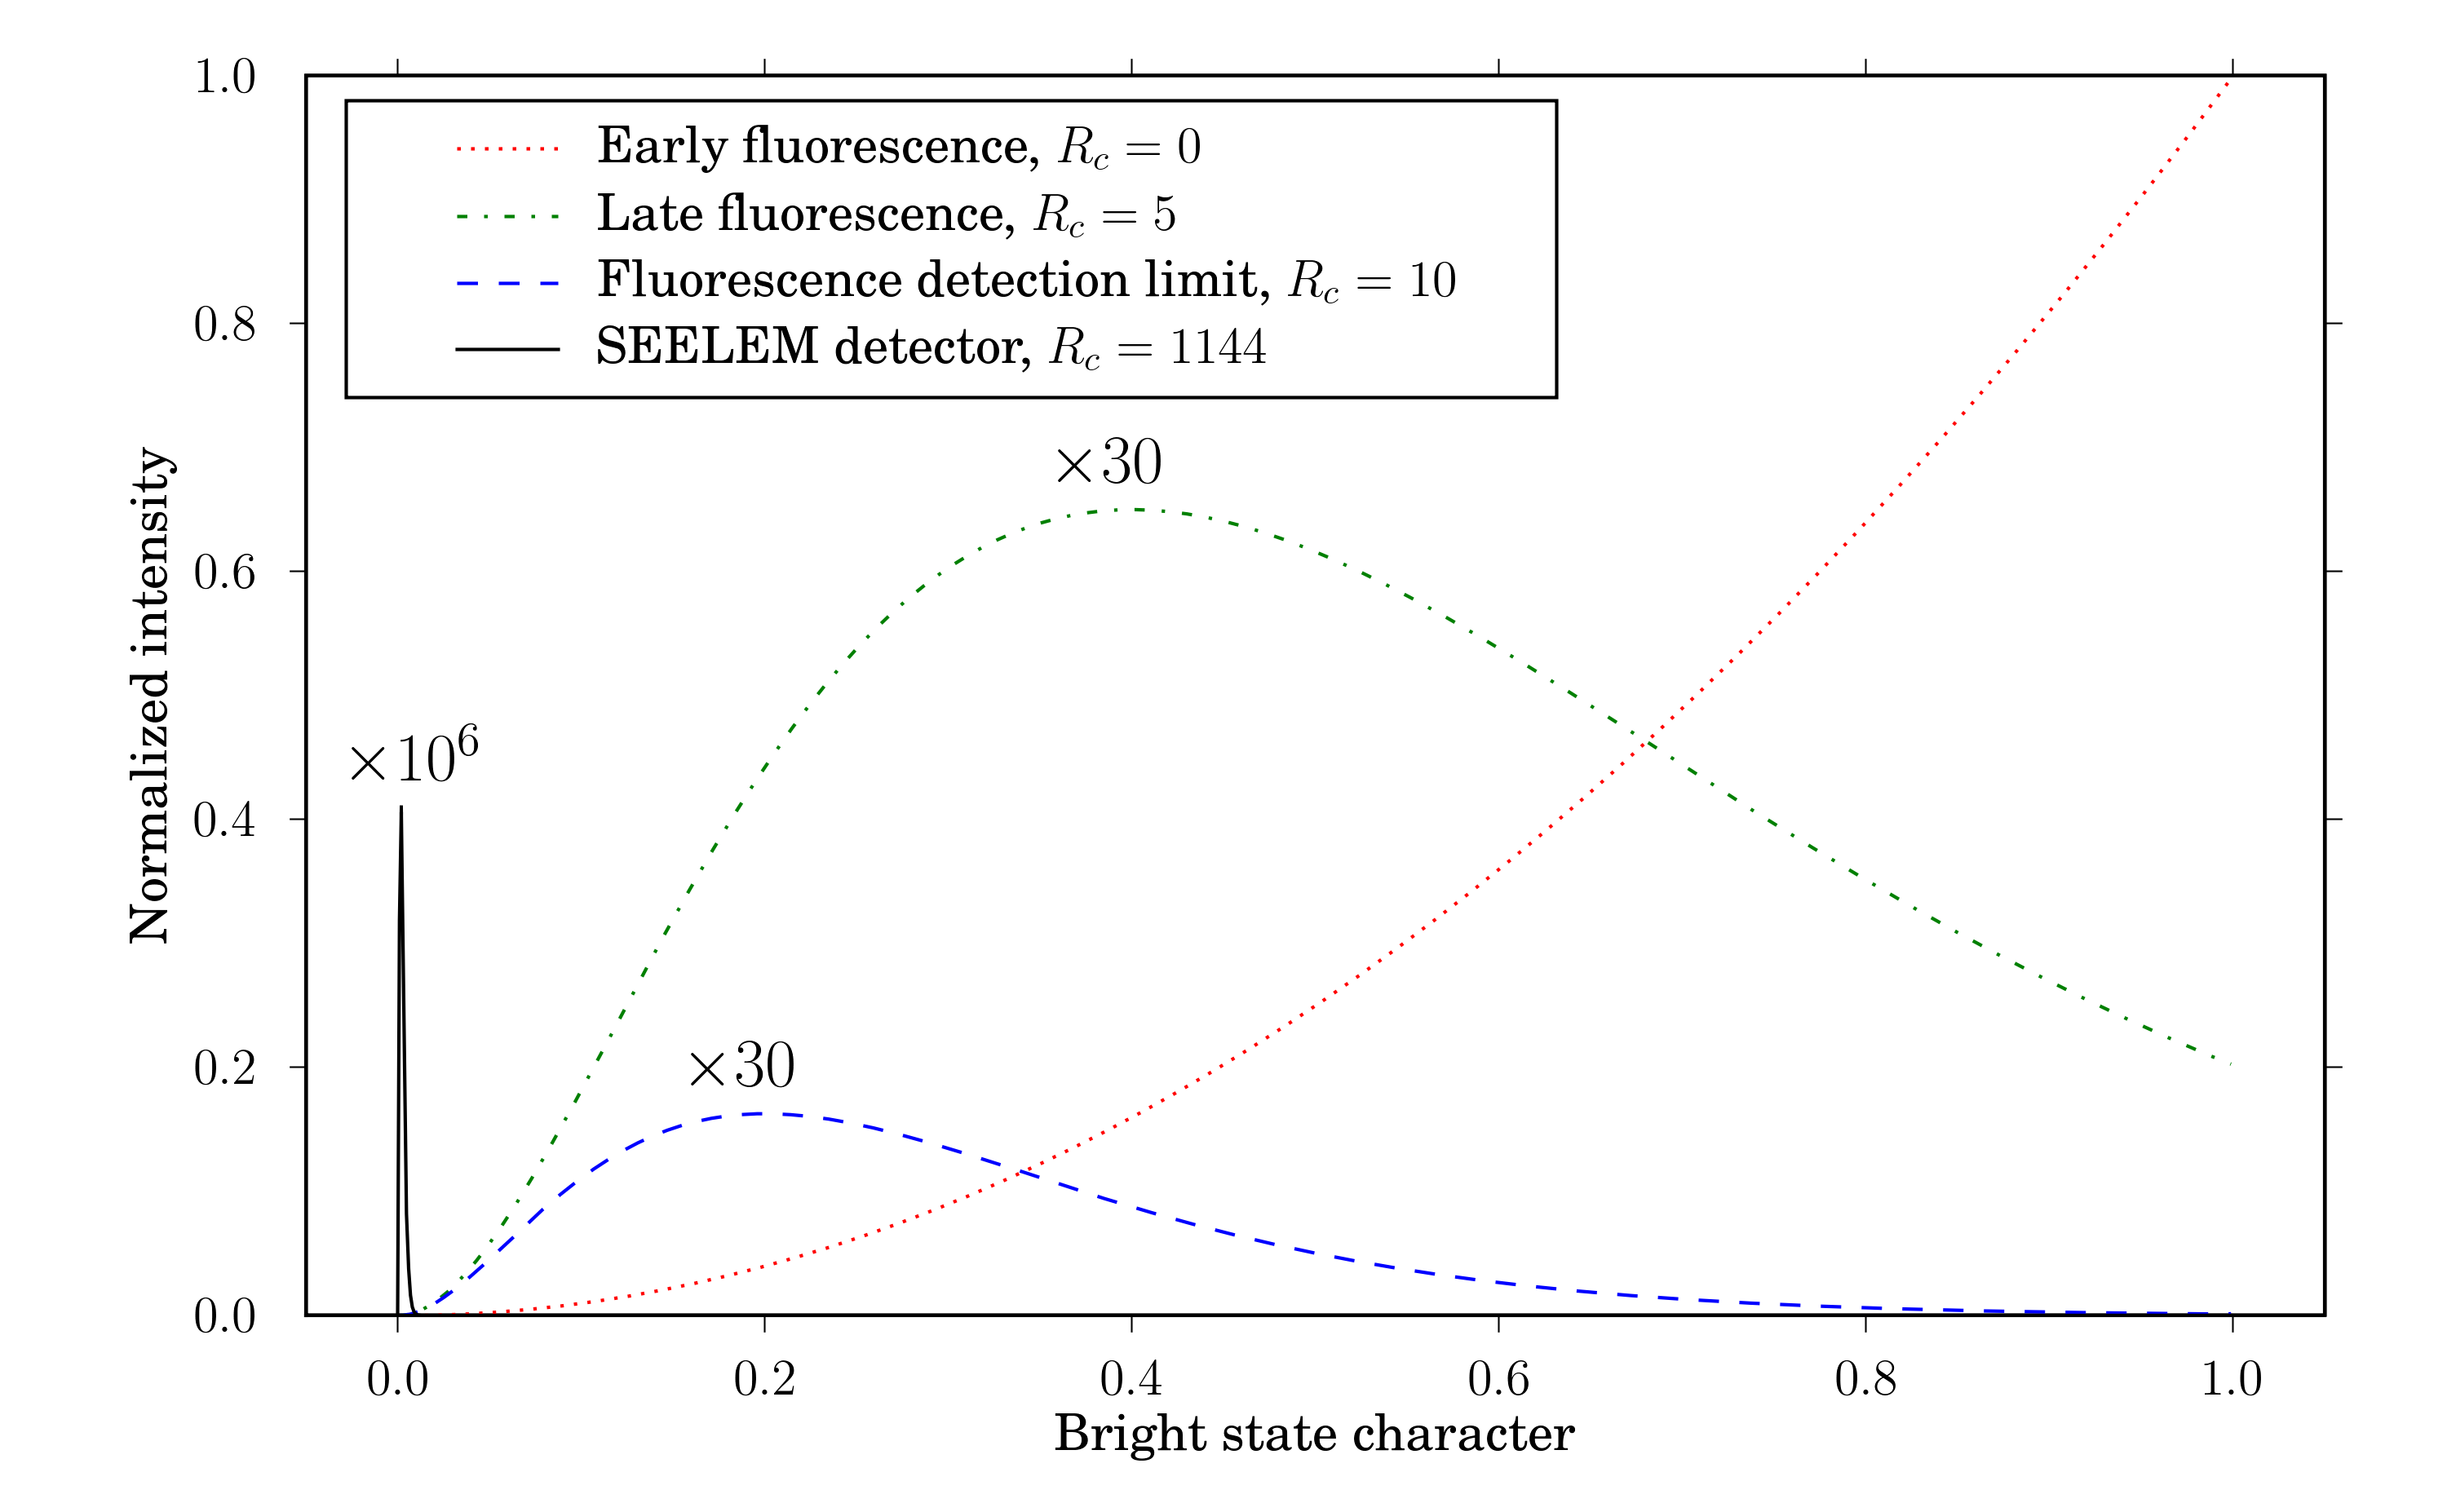
\includegraphics[width=7.5in,angle=90]{intensity-at-rc.png}
\end{figure}

Figure \ref{fig:int-at-rc} shows the dependence of fluorescence
intensity on bright state character for several values of $R_c$.  At
early fluorescence times ($\sim \tau_s$), the fluorescence intensity
is greatest for states with large amounts of bright state character
($2/R_c > 1$).  At a delay of $5 \tau_s$, the fluorescence intensity
equation discriminates against states with large amounts of bright
state character, since molecules in such states have already
fluoresced with high probability.  States with small amounts of bright
state character are also discriminated against -- molecules in these
states have a low probability of fluorescing at the time under
consideration.  The fluorescence intensity is thus ``tuned'' to a
particular value of bright state character at every time delay $R_c$,
according to Equation \ref{eq:am-max}.

Note that the intensity expression used here does not account for
molecules leaving the field of view of the fluorescence detection
optics.  We consider only the distribution of bright state character
\emph{among molecules remaining in the field of view at time $R_c$}.
However, since there is no momentum transfer from the excitation
photon to the molecule, the rate of molecules exiting the field of
view is independent of bright state character.  Therefore,
simple reasoning according to the above intensity formulas will be
correct as long as we discuss fluorescence intensities only in terms
of ratios.

To foster a more concrete discussion, consider our experiments on
intersystem crossing in acetylene.  For the $S_1$ electronic state,
$\tau_s=270$ ns.  In our apparatus, the field-of-view of the
fluorescence detection optics is several mm, which amounts to a
maximum viewing time of 3 $\mu$s, about $10\tau_s$, for molecules in
the molecular beam with a velocity of $10^3$ m/s.  At times later than
$10\tau_s$, there are simply no molecules left to observe in the
fluorescence field of view.  This places an upper limit on the value
of $R_c$ that can be examined in our fluorescence experiments.  Figure
\ref{fig:int-at-rc} shows the intensity equation for the limit of
fluorescence detection, $10\tau_s$.

The SEELEM detector used in our experiments detects metastable
molecules after a 309 $\mu$s flight time.  If we set aside some
particularly interesting aspects of SEELEM detectivity and consider
only its detection sensitivity to bright state character, we arrive at
the following equation for SEELEM detection probability (Chapter 2,
equation 28):
\begin{equation}
  \label{eq:seelem-prob-s}
  P_{SEELEM}^{(s)} \propto a_m^4 \; \exp \left( -R_c \, a_m^2 \right).
\end{equation}
(This is a good approximation to its overall detection sensitivity,
including $T_3$, in the weak coupling limit.)  The SEELEM detection
probability equation above has the same functional form as the
Equation \ref{eq:int-m}.  Thus, the SEELEM detector may be viewed in
this limited sense as an extreme discriminator for states with small
amounts of bright state character.

Acetylene molecules in our apparatus are detected after an average
flight time of 309 $\mu$s, yielding an $R_c$ value of $1144$ for the
SEELEM detector.  This corresponds to a maximum detection probability
for states with $0.17\%$ bright state character.

\subsection{Delayed fluorescence of a two-level system}

Our next step is to examine the changing characteristics of a
fluorescence intensity distribution as we increase the time delay
$R_c$.  We model the interaction between a bright state and an
ensemble of dark states by generalizing from a two-level system.
Consider a Hamiltonian with only one dark state.  Define the two mixed
states $\ket{m=1,2}$ as
\begin{equation}
  \begin{split}
    \ket{1} &=  (1 - \alpha^2)^{1/2} \ket{s} + \alpha \ket{t}\\
    \ket{2} &= -\alpha \ket{s} + (1 - \alpha^2)^{1/2} \ket{t}.
  \end{split}
\end{equation}
The fluorescence intensity of both states, relative to a pure bright
state, is
\begin{equation}
  \begin{split}
    I_1 &= \frac{(1 - \alpha^2)^2}{\tau_s} \; \exp 
          \left[
            - R_c \, (1 - \alpha^2)
          \right]\\
    I_2 &= \frac{\alpha^4}{\tau_s} \; \exp 
          \left[
            - R_c \, \alpha^2
          \right],
  \end{split}
\end{equation}
and the ratio of the fluorescence intensities changes with time as
\begin{equation}
  I_{12} = I_1 / I_2 = 
  \left(
    \frac{(1 - \alpha^2)}{\alpha^2}
  \right)^2
  \exp
  \left[
    - R_c \, (1 - 2\alpha^2)
  \right].
\end{equation}
The fluorescence intensity ratio may be used to write an equation for
the dependence of average intensity on $R_c$.
\begin{equation}
  \label{eq:ratio}
  \braket{I_{LIF}} = 
  \frac{\Delta E_{12}}{2} \,
  \left(
    \frac{I_{12}-1}{I_{12}+1}
  \right)
\end{equation}
Figure \ref{fig:ratio} shows the dependence of center-of-gravity on
the intensity ratio $I_{12}$.

\begin{figure}
  \caption{Center of gravity as a function of the intensity ratio
    $I_1$:$I_2$ for a two-state system.  At $t=0$, the initial center
    of gravity is a function of the mixing amplitude $\alpha$.  The
    center of gravity then shifts with the changing intensity ratio as
    delay time is increased, arriving at a limiting value of $-\Delta
    E_{12}/2$.}
  \label{fig:ratio}
  \centering
  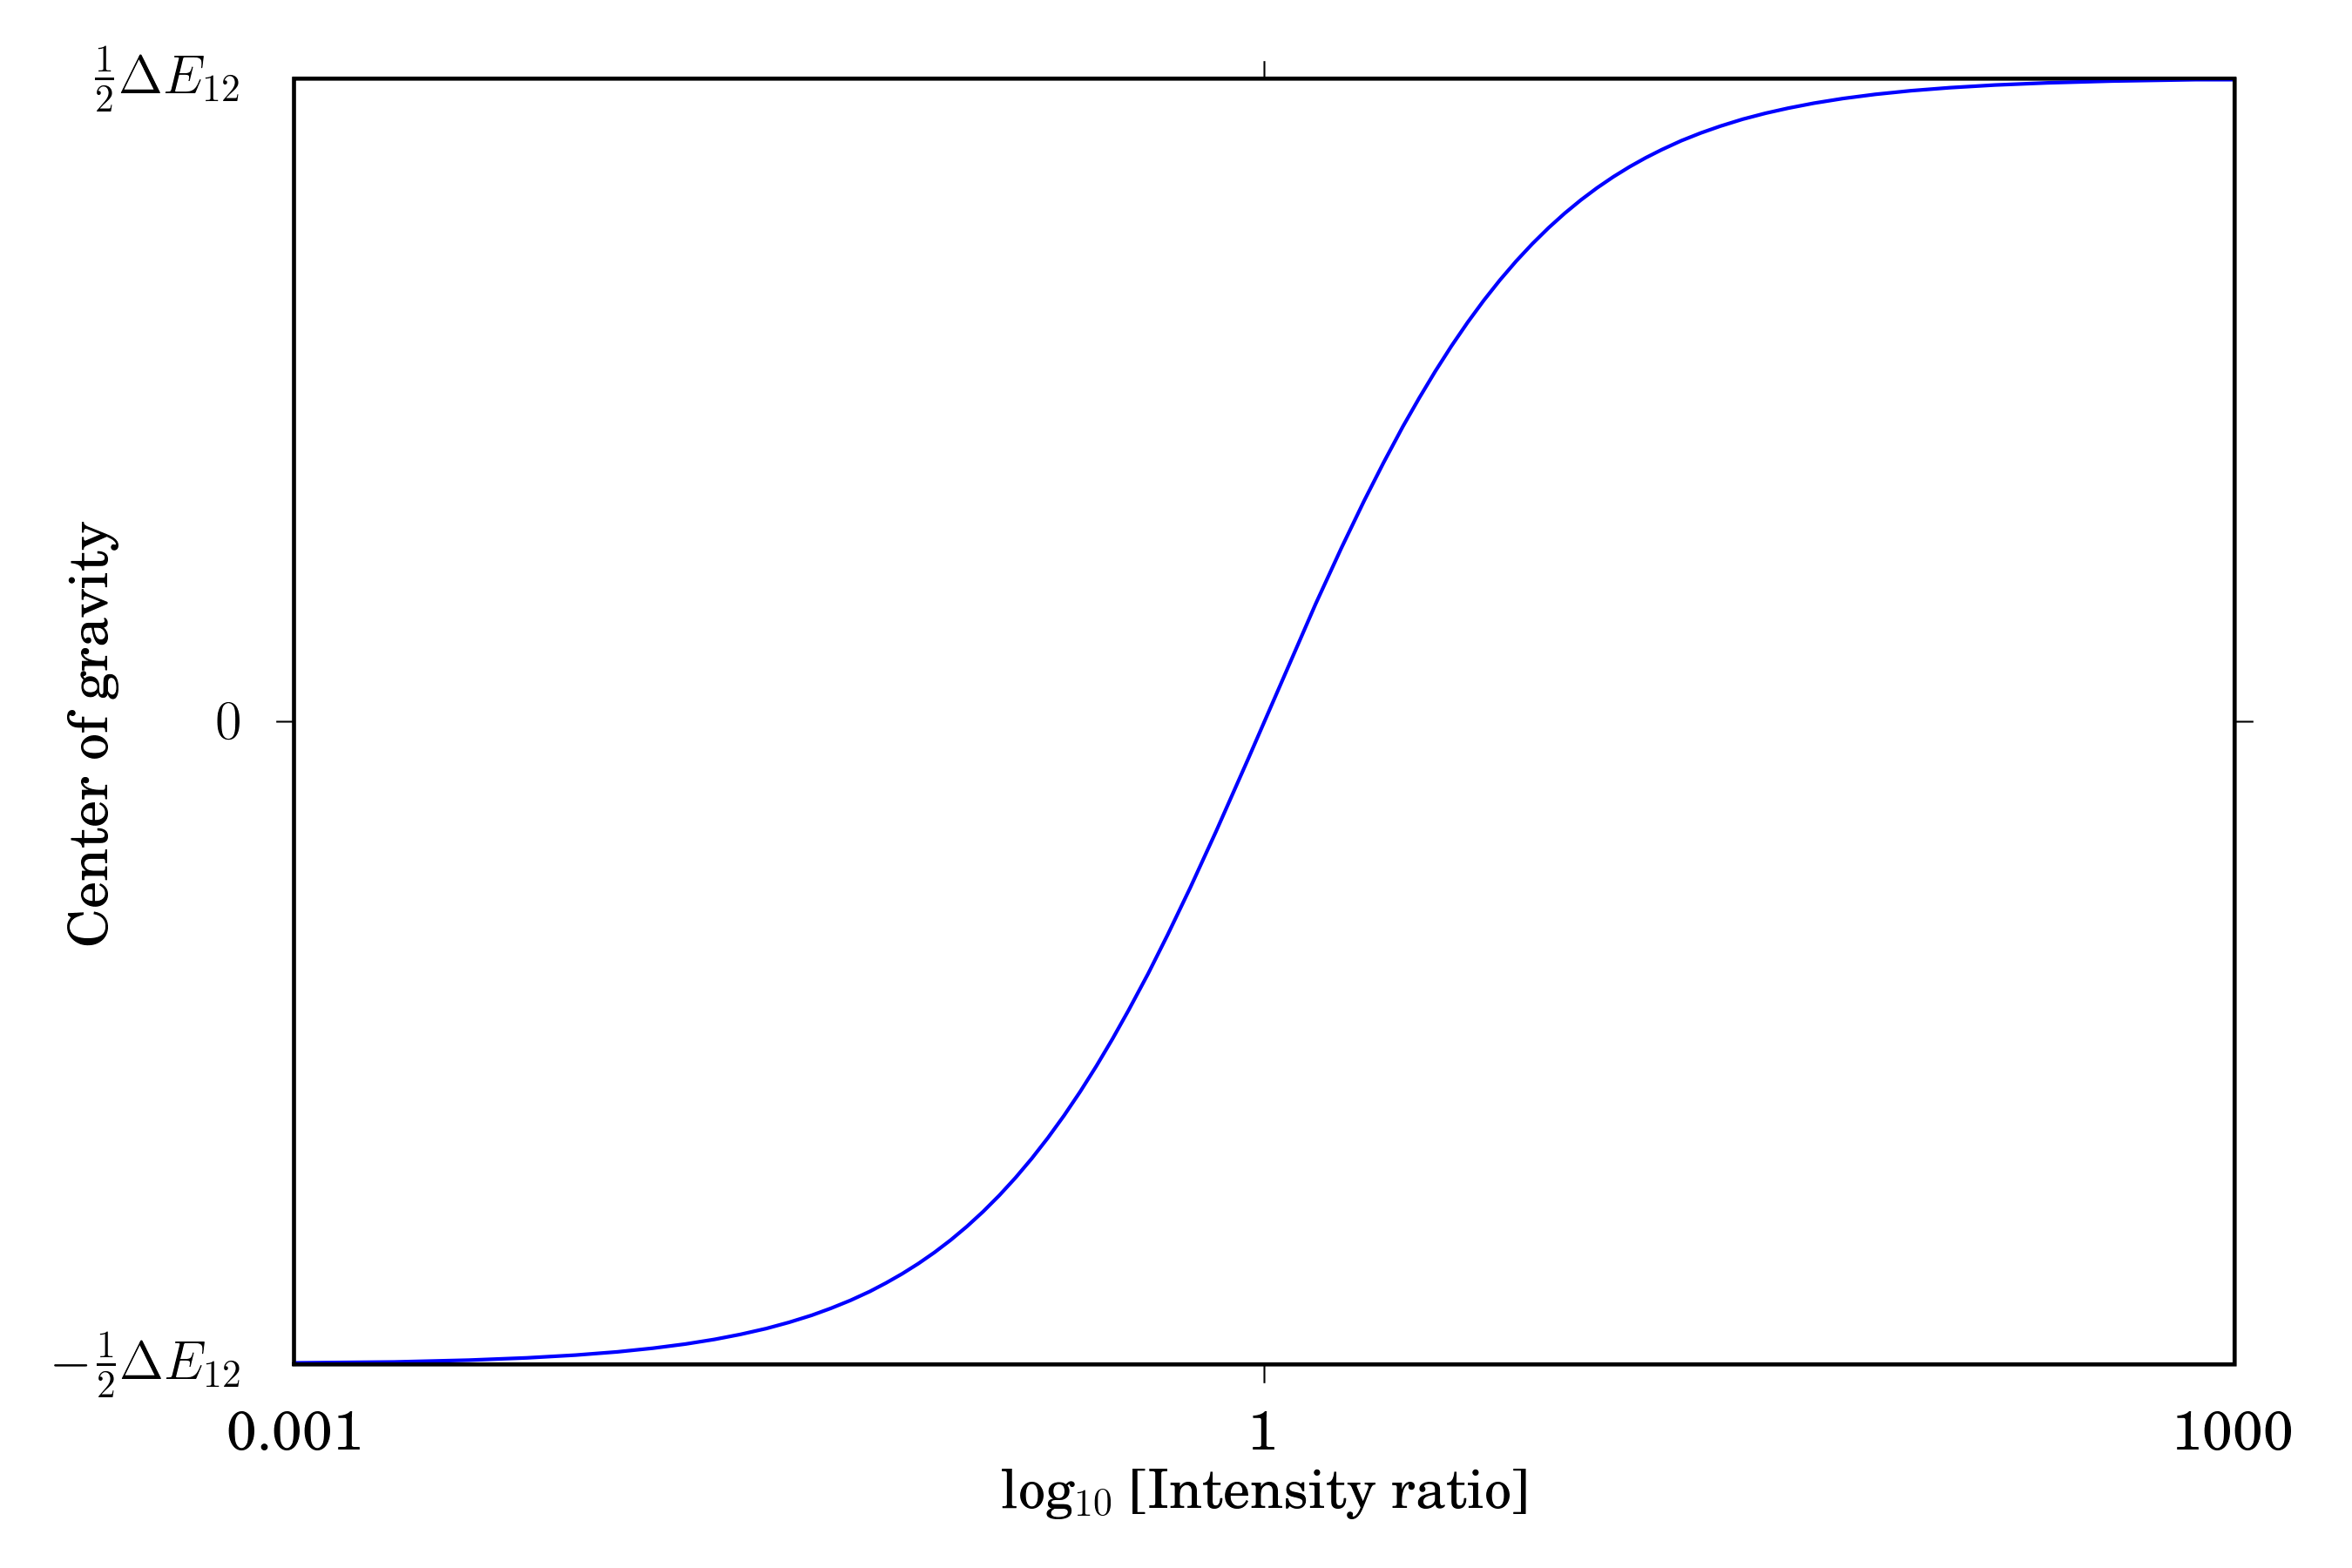
\includegraphics[width=6in]{cog-from-ratio.png}
\end{figure}

The initial intensity ratio at time $R_c=0$ is just
\begin{equation}
  I_{12} = 
  \left(
    \frac{(1 - \alpha^2)}{\alpha^2}
  \right)^2.
\end{equation}
From this, the initial center of gravity can be found according to
Equation \ref{eq:ratio} or Figure \ref{fig:ratio}.  At large values of
$R_c$, the intensity ratio decreases to zero as $I_1 \ll I_2$, as long
as the states are not 50:50 mixed.  As the ratio decreases to zero,
the center of gravity approaches $-\Delta E_{12} / 2$.  The
development of intensity ratios and the consequent shift in center of
gravity are shown in Figure \ref{fig:cog-devel}.  One interesting
aspect of the center of gravity shift shown in the figure is the rapid
onset of the shift at small mixing coefficients.  

\begin{figure}
  \caption{(Top) Time development of the relative intensity ratio for
    a two state system. (Bottom) Time development of the center of
    gravity for a two state system.}
  \label{fig:cog-devel}
  \centering
  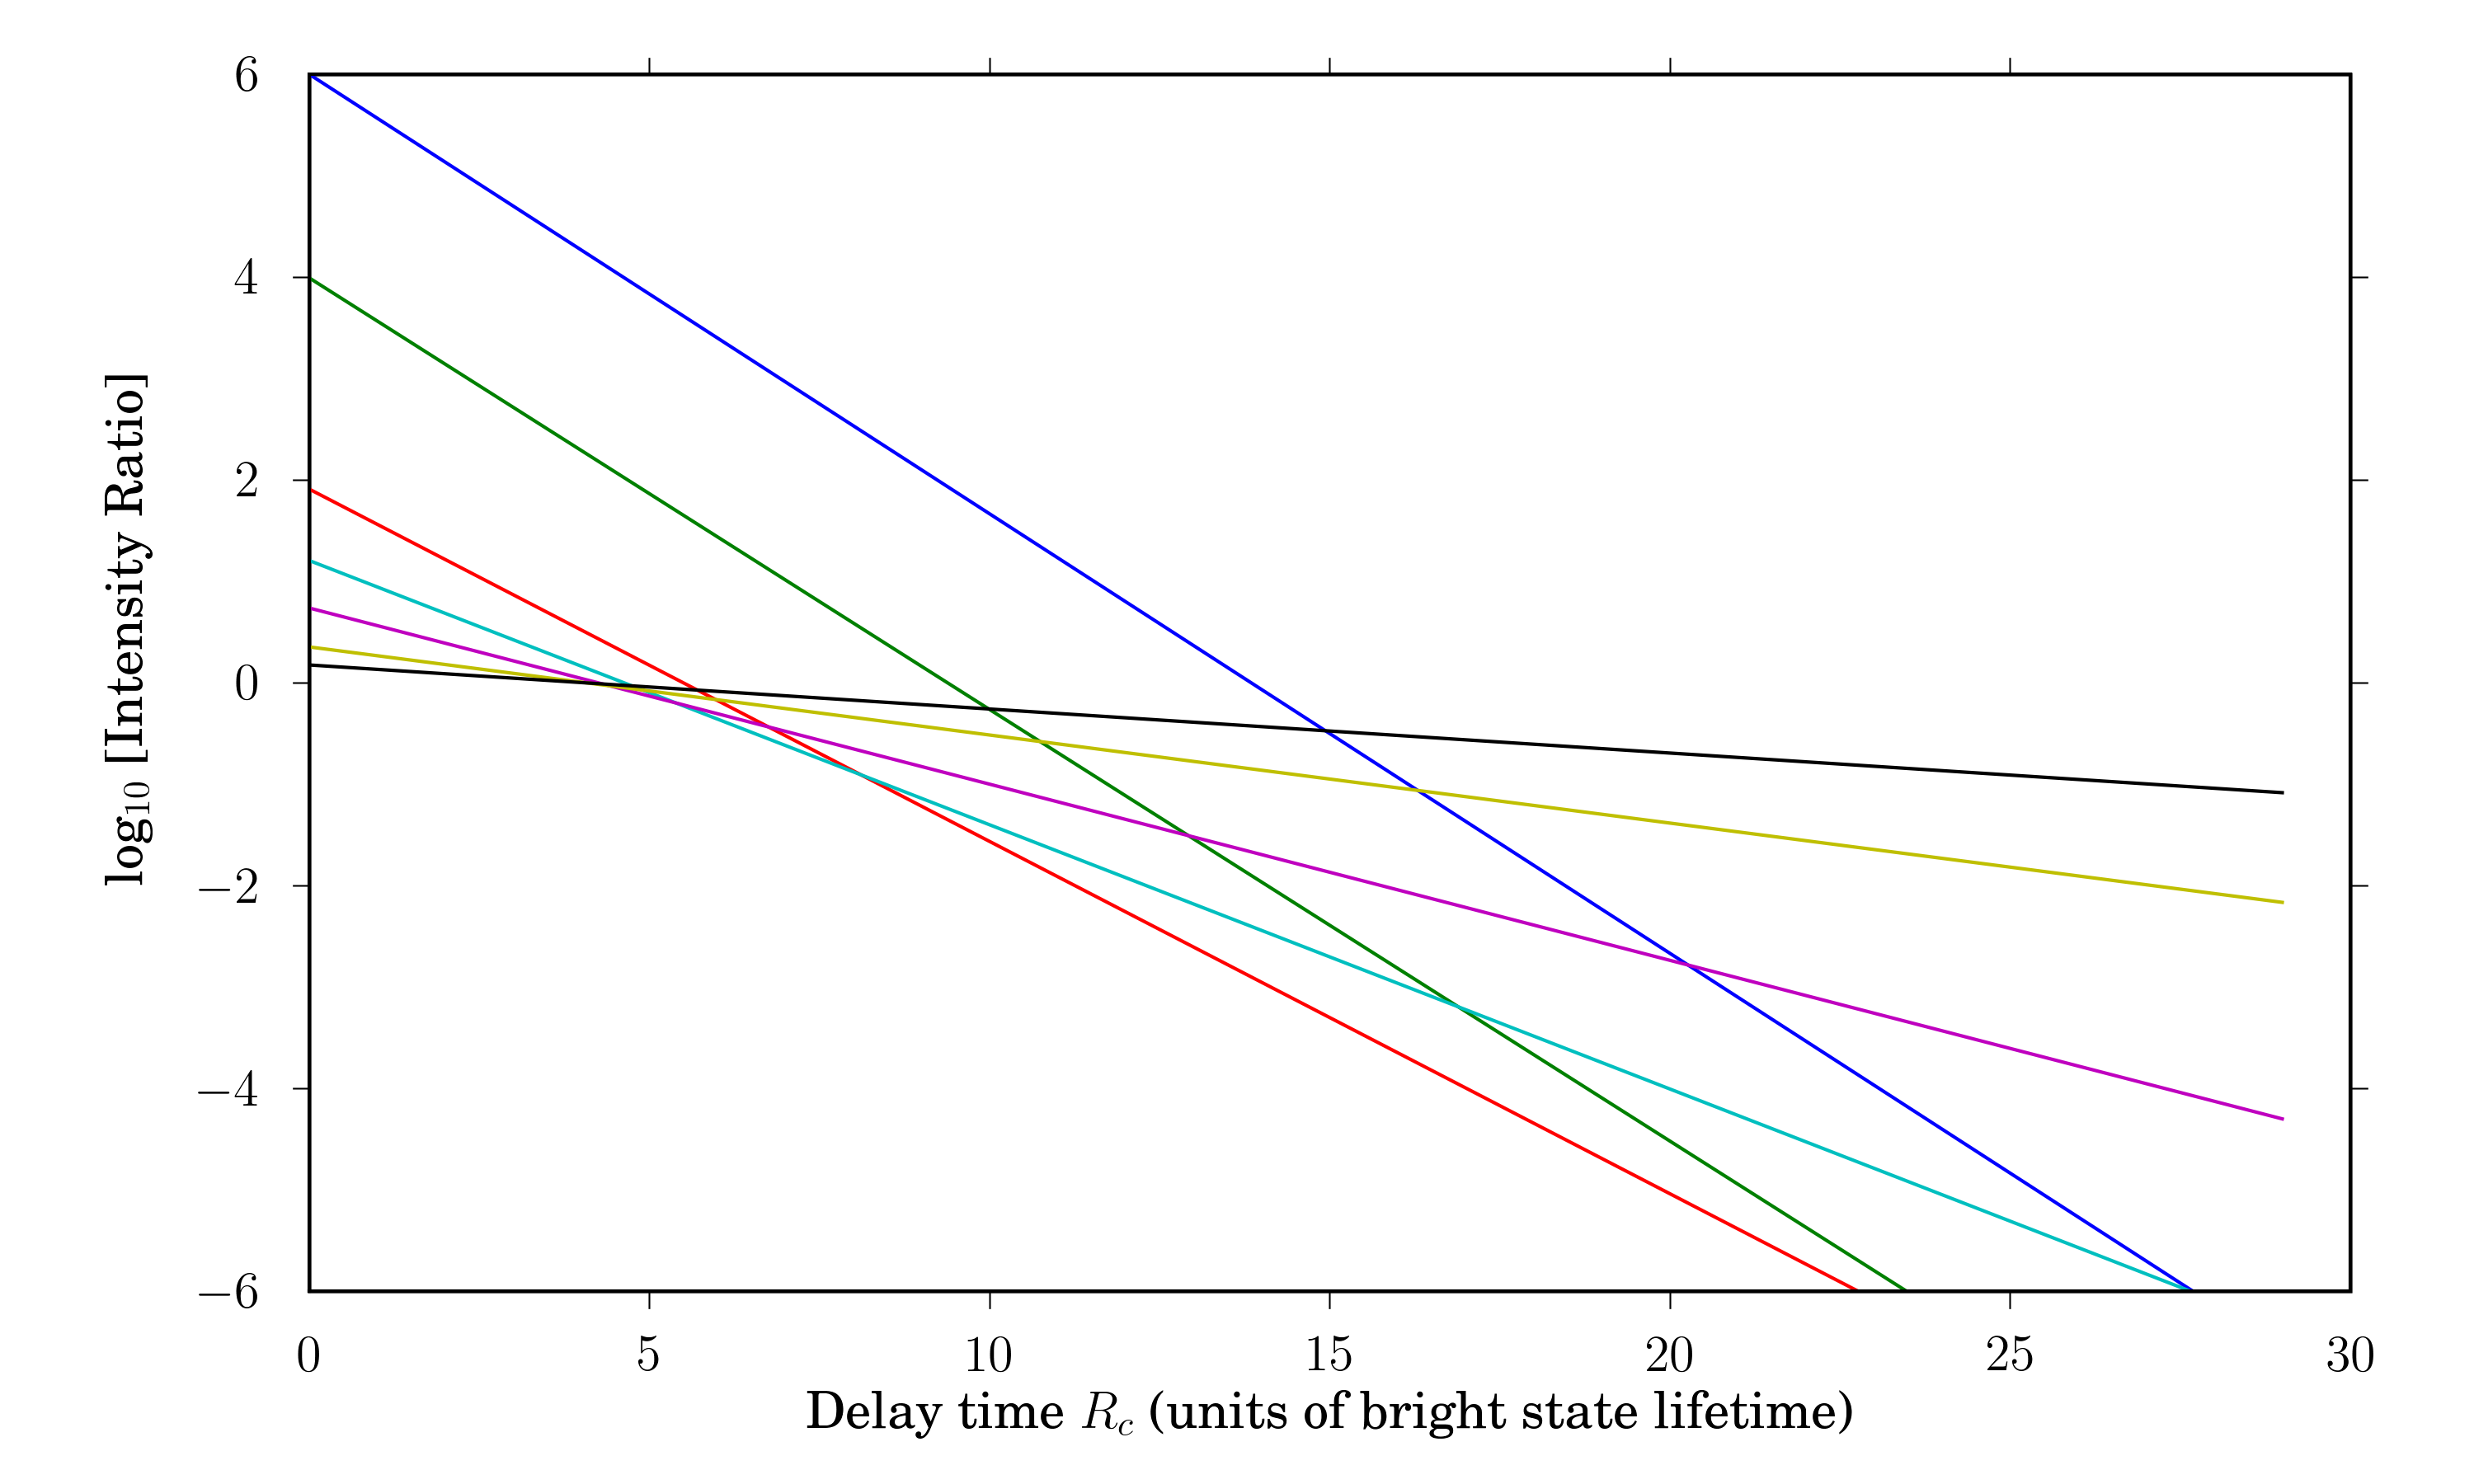
\includegraphics[width=6in]{ratio-development.png}
  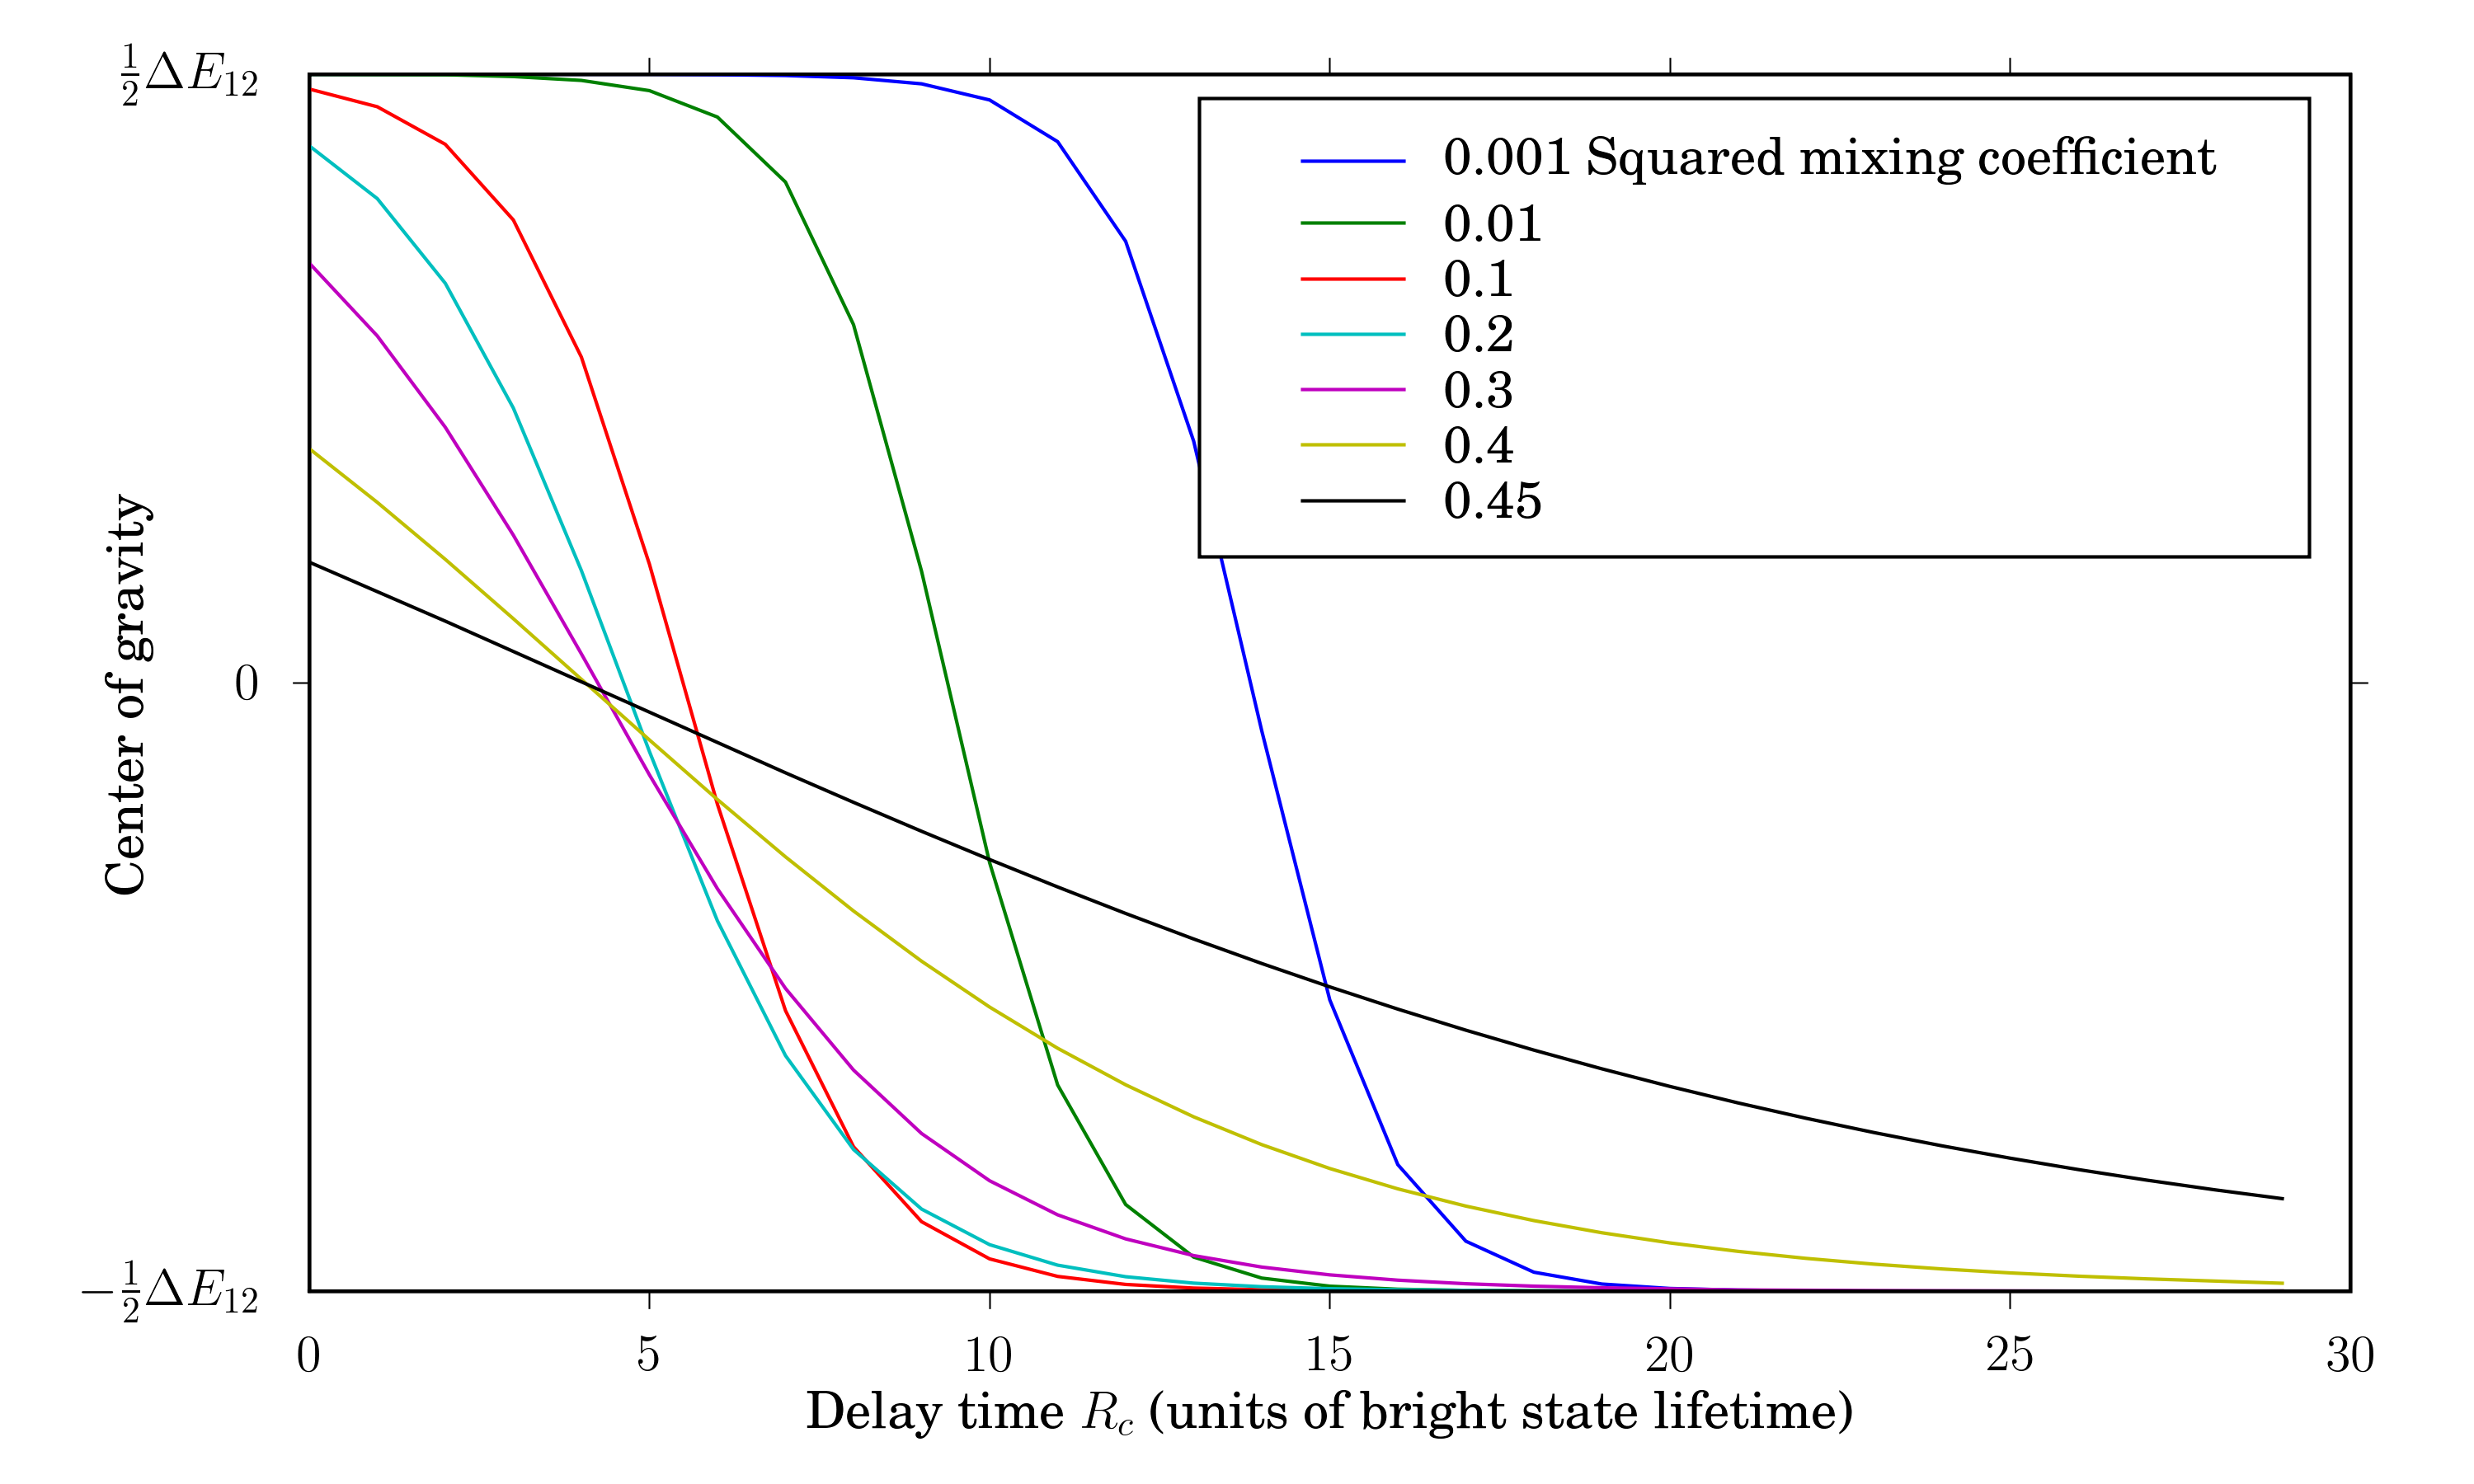
\includegraphics[width=6in]{cog-development.png}
\end{figure}

\subsection{Delayed fluorescence of a series of rotational
  transitions}

Information about the relative B-value of a mediating level can be
recovered by studying the statistical properties of delayed
fluorescence as a function of rotational quantum number.

\POINT{Review components and selection rules.}  We take as a model
system a series of equally spaced bright state transitions with
increasing rotational quantum number $J$.  The total bright$\sim$dark
coupling strength for each transition is function of the energy
separation between the bright state $\ket{s;J}$ and three components
of the non-local mediating level: $F_1$, $\ket{\ell;J-1}$; $F_2$,
$\ket{\ell;J}$; and $F_3$, $\ket{\ell;J+1}$.

\begin{figure}
  \caption{ Reduced term value plot of the three singlet$\sim$triplet
    roational components permitted by the spin-orbit operator in
    Hund's case ($b$).  The $F_1$ component corresponds to  }
  \label{fig:components}
  \centering
  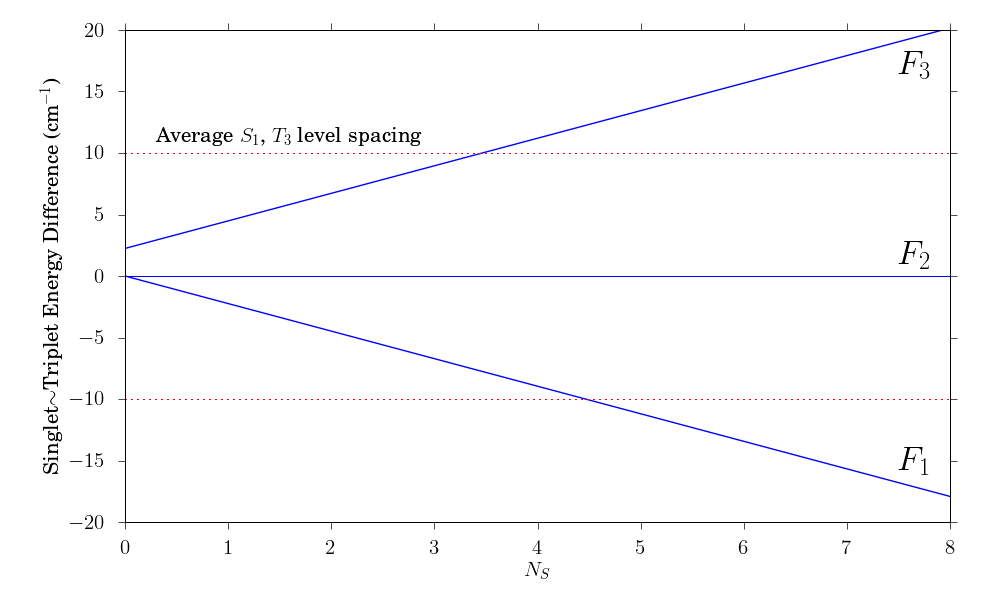
\includegraphics[width=6in]{f-components.png}
\end{figure}

To a very good approximation the total first-order spin-orbit matrix
element between two rovibrational states is given by the product of
three factors: an electronic spin-orbit matrix element, a vibrational
overlap factor, and a rotational factor arising from angular momentum
coupling rules.  The rotational factors are given for the general case
of polyatomic molecules by Stevens and Brand \cite{stevens73}.  

Plots of the spin-orbit rotational factors are presented for singlet
levels having $K$=0 (Figure \ref{fig:rotational-factors-0}), $K$=1
(Figure \ref{fig:rotational-factors-1}), and $K$=2 (Figure
\ref{fig:rotational-factors-2}).

The rotational dependence of energy differences for the three
components is
\begin{equation}
  \Delta E_{s\ell}(J) = 
  \begin{cases}
    \Delta B_{s\ell}J(J+1) + 2B_{\ell}J           & F_1 \text{ component}\\
    \Delta B_{s\ell}J(J+1)                      & F_2 \text{ component}\\
    \Delta B_{s\ell}J(J+1) - 2B_{\ell}J - 2B_{\ell} & F_3 \text{ component}.\\
  \end{cases}
\end{equation}
We simplify the above formulas by considering the \emph{average}
energy difference, taking all components into account.  Giving equal
weights to all components, the average energy separation is
\begin{equation}
  \Delta E_{s\ell}(J)_{\text{ave}} = \Delta B_{s\ell}J(J+1) - \frac{2}{3}B_{\ell}.
\end{equation}
We define a mixing coefficient $\alpha_{s\ell}$ between the bright
state and the three components of the mediating level.  The mixing
coefficient can be related to $\Delta E_{s\ell}$ using second order
perturbation theory.  Introducing the average spin-orbit matrix
element $H_{s\ell}$ for the three rotational components, the relation
is $\alpha_{s\ell}(J) = H_{s\ell} / \Delta E_{s\ell}(J)$.  The
relative strengths of the three components are given by simple
formulas, which can be found in the literature.  We find that the
functional dependence of the mixing coefficient between the bright
state and the mediating components is
\begin{equation}
  \alpha_{s\ell}(J) = \frac{H_{s\ell}}{\Delta B_{s\ell}J(J+1)}.
\end{equation}

\POINT{Present rotational factors for first-order spin-orbit
  coupling.}

\begin{figure}
  \caption{}
  \label{fig:rotational-factors-0}
  \centering
  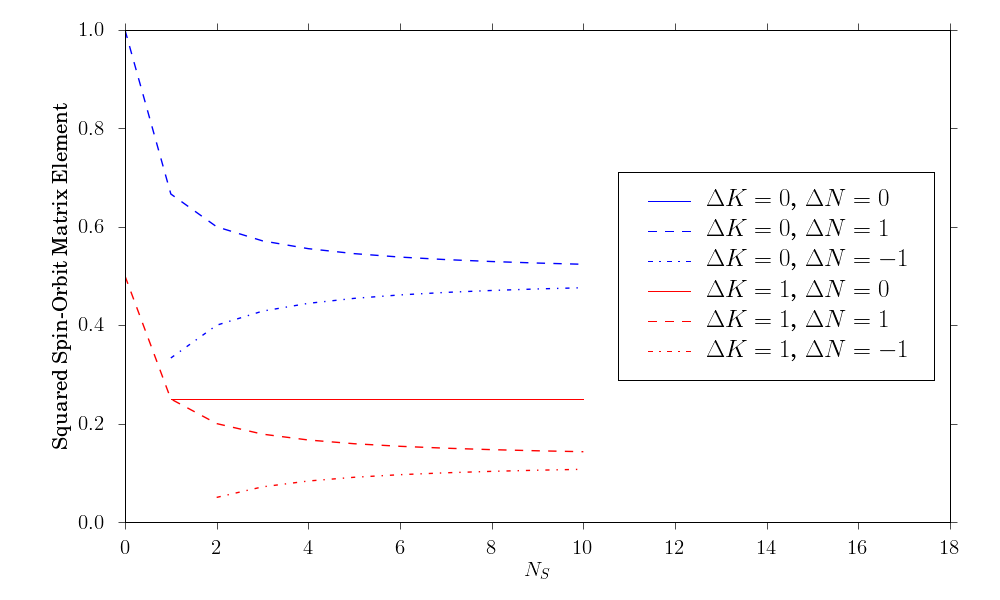
\includegraphics[width=6in]{rotational_factors_k0.png}
\end{figure}

\begin{figure}
  \caption{}
  \label{fig:rotational-factors-1}
  \centering
  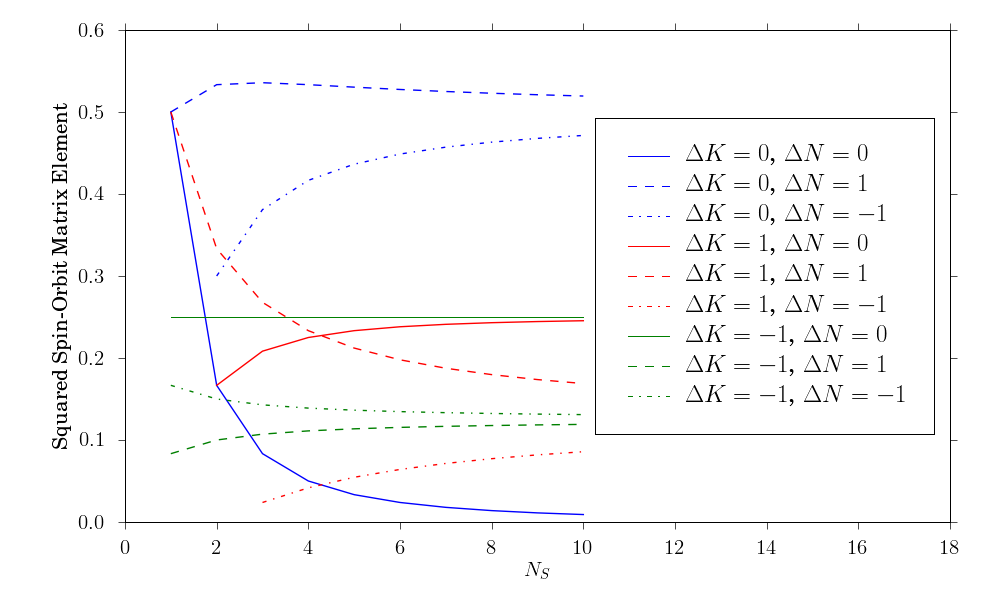
\includegraphics[width=6in]{rotational_factors_k1.png}
\end{figure}

\begin{figure}
  \caption{}
  \label{fig:rotational-factors-2}
  \centering
  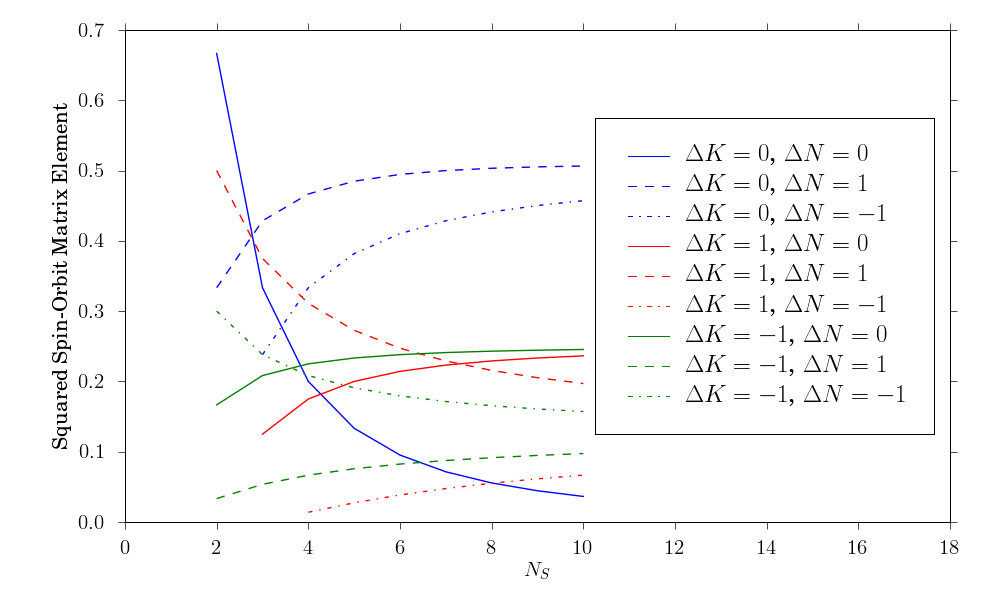
\includegraphics[width=6in]{rotational_factors_k2.png}
\end{figure}

\section{Experiment}

\TODO{Adapt this from paper.}

SEELEM is a versatile and sensitive technique for investigating
``dark'' (weakly-fluorescing) metastable molecules produced via laser
excitation.1-6 In the SEELEM experiment, a molecular beam of acetylene
is excited by a $\sim$5 ns pulsed laser into spin-rotation-vibration
eigenstates of metastable electronic states via weak, nominally
forbidden transitions. After excitation, the long-lived species must
travel 35 cm before colliding with an Au metal detector surface, where
an electron is ejected in a de-excitation process. Two criteria must
be met for electron ejection by a metastable species. First, the
vertical electronic energy of the metastable approaching the surface
must exceed the work function of the metal ($\Phi$Au = 5.1
eV). Second, the radiative lifetime of the detected metastable
eigenstate ($\tau_\text{rad}$) must exceed the flight time from the
point of laser excitation to the SEELEM surface ($\Delta$t=300
$\mu$s).

A sample of acetylene (BOC gases) at a backing pressure of one
atmosphere was pulsed through a 0.5 mm diameter nozzle operating at 10
Hz into a diffusion pumped vacuum chamber at $\sim$5x10-5 torr.  An Nd:YAG
pumped, frequency-doubled dye laser (220 nm) excited the acetylene
molecules in the pulsed jet expansion 2 cm downstream from the nozzle
orifice. UV-LIF was detected perpendicular to the plane defined by the
intersection of the pulsed molecular and laser beams using f/1.2
collection optics, a fluorescence filter (UG-11) to reduce scattered
laser light, and a PMT (Hamamatsu model R375). The fluorescence signal
was averaged by a boxcar integrator and recorded. For SEELEM
detection, the excited molecules in the pulsed expansion passed
through a conical skimmer (3mm diameter) to form a collimated
molecular beam, which traveled into a differentially pumped detector
chamber maintained at $\sim$4x10-7 torr, and collided with a heated (300
C) Au metal surface 35 cm downstream from the point of laser
excitation. The SEELEM detector was identical to that used in the
previously described apparatus with Au foil ($\Phi$ = 5.1 eV) as the
metal surface.  Particle counting techniques, including a multichannel
scalar (Oxford Tennelec Nucleus Inc. MCS-II v2.091) were used to
record laser-excited metastable counts as a function of laser
frequency, along with the simultaneously recorded LIF spectra. Both
SEELEM and LIF signals were averaged over 100 laser shots / data
point.


\section{Investigation of several $2^13^1B^2$ and $3^2B^2$ polyad
  members}

\TODO{Make survey figure showing the energy of all investigated bands,
  overlayed on acetylene LIF spectrum.}

\subsection{Results}

\TODO{Adapt the following from the paper.}

Figure \ref{fig:spectrum-2131b2}(a) shows the SEELEM (plotted upward)
and LIF (plotted downward) spectra for the $\tilde{A}^1A_u \leftarrow
\tilde{X}^1\Sigma_g$ nominal $2^13^14^2$ $K_a$=1 $\leftarrow$ $0_0$ Q
and R branch rovibronic transitions of acetylene near 46195 cm-1. The
SEELEM and LIF spectra are very similar for this band in terms of both
frequencies and relative intensities, with the exception of the
anomalously weak LIF Q(1) feature. Each SEELEM feature in the spectrum
is localized in energy near an LIF partner feature. No splitting of
the rotational lines in the LIF spectrum is observed at the 0.06 cm-1
resolution.

Figure \ref{fig:spectrum-2131b2}(b) presents the SEELEM / LIF spectra
for the $\tilde{A}^1A_u \leftarrow \tilde{X}^1\Sigma_g$ nominal
$2^13^16^2$ $K_a$=1 $\leftarrow$ $0_0$ P, Q and R branch transitions
near 46090 cm-1. The SEELEM spectrum of $2^13^16^2$ is remarkably different
from that of 213142. The overall SEELEM signal in $2^13^16^2$ is weaker
than that of $2^13^14^2$ by nearly a factor of 3, even though the LIF
intensity in $2^13^16^2$ is a factor of 3 stronger than that of 213142.  In
213162, the SEELEM features are not well correlated in intensity with
the corresponding features in LIF. In fact, in several cases where a
strong LIF feature appears, the partner SEELEM feature is near or
completely below the noise level. The observed pattern of SEELEM
features in $2^13^16^2$ suggests a significant J' dependence to the SEELEM
activity, and hence, to the interaction of the bright singlet state,
S1, with the perturbing triplet state, T3.

\begin{figure}
  \caption{
    % Simultaneously recorded LIF and SEELEM spectra of the
    % acetylene $2^1_0V^1_04^2_0K^1_0$ and $2^1_0V^1_04^2_0K^1_0$
    % $\tilde{A}^1A_u \leftarrow \tilde{X}^1\Sigma_g$ transitions.  
    % Ripped off from paper.
    (a) Simultaneously recorded surface electron ejection by laser 
    excited metastables (SEELEM, upper trace) and ultraviolet 
    laser-induced fluorescence (UV-LIF, lower trace) spectra of the 
    $2^13^14^2$ $K_a$=1 sublevel of the $\tilde{A}^1A_u \leftarrow
    \tilde{X} ^1\Sigma_g^+$ electronic transition.  (b) P, Q, and R
    branch features of the SEELEM and LIF spectra of the $2^13^16^2$ 
    $K_a$=1 sublevel. The weak Q branch features, which are overlapped 
    with the R branch features of $2^13^16^2$ $K_a$=1, belong to a 
    sublevel of a different polyad.
  }
  \label{fig:spectrum-2131b2}
  \centering
  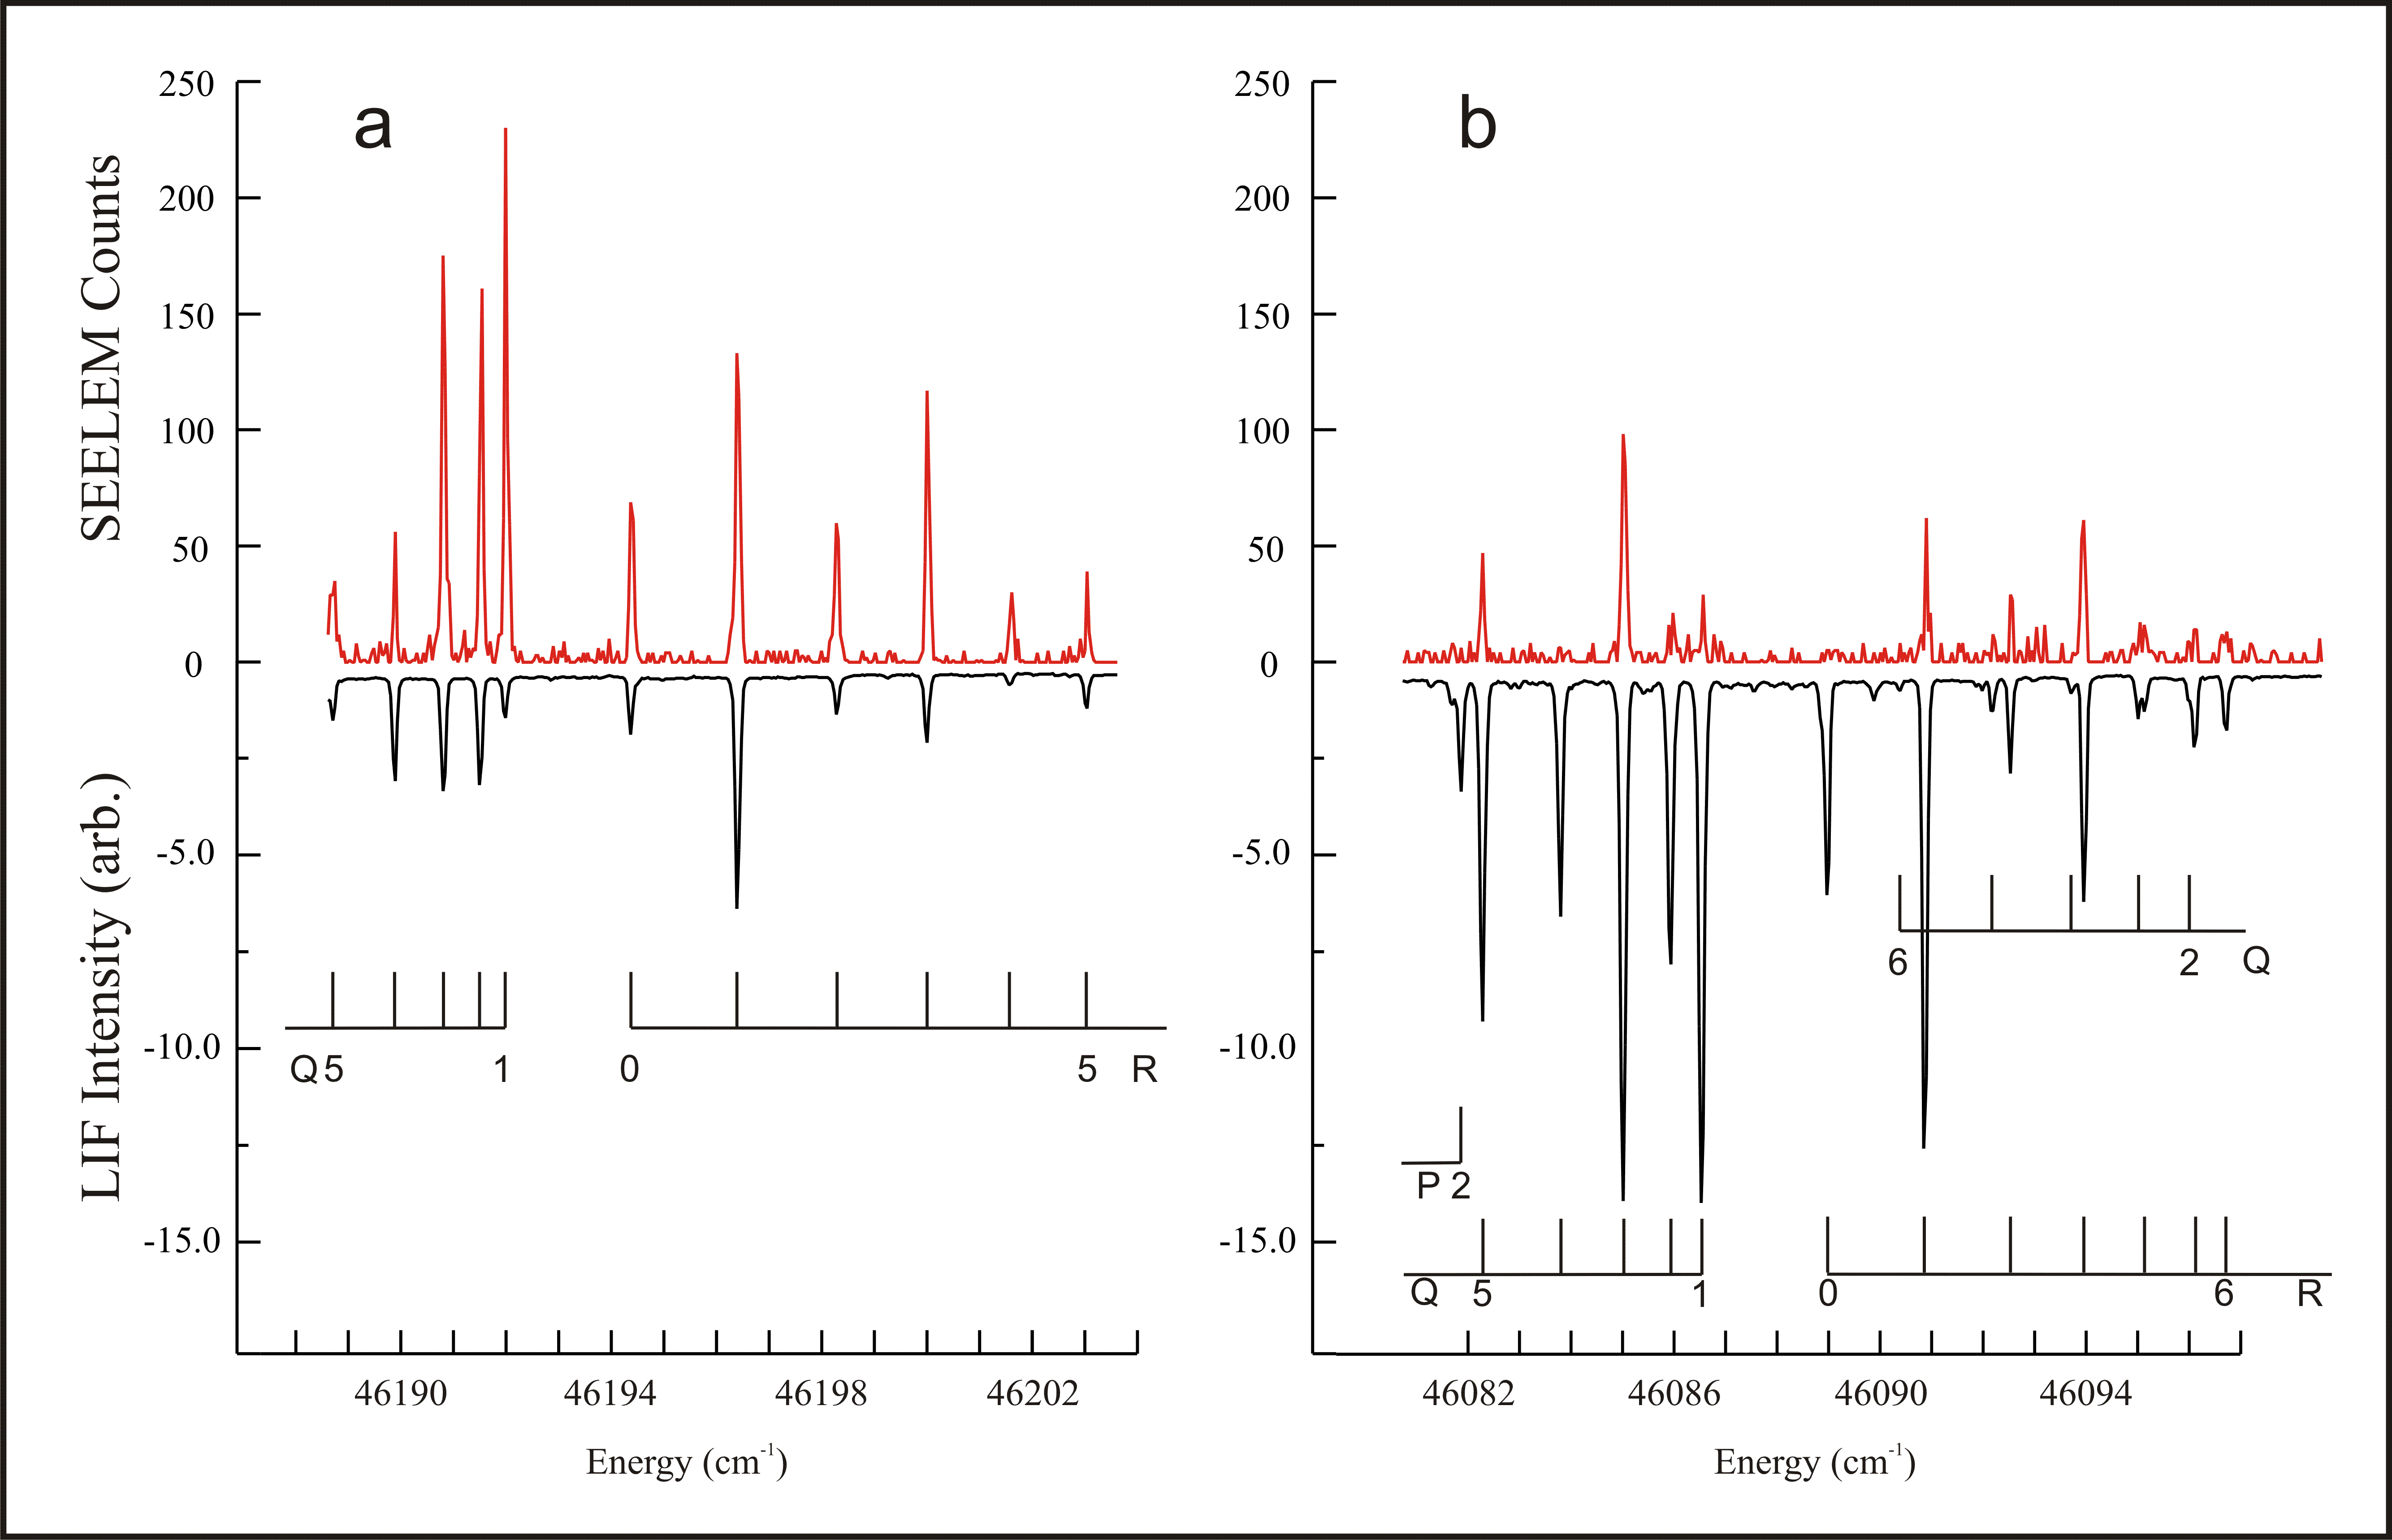
\includegraphics[width=7.5in,angle=90]{spectrum-2131b2.png}
\end{figure}

\POINT{SEELEM spectrum of $3^2 4^2$ with lone SEELEM peak in band gap
  (December 2006, p.86 of 9/2006--1/2007 notebook.)}  This spectrum is
shown in Figure \ref{fig:spectrum-32b2}.

\begin{figure}
  \caption{
    % Simultaneously recorded LIF and SEELEM spectra of the
    % acetylene $V^2_04^2_0K^1_0$ $\tilde{A}^1A_u \leftarrow
    % \tilde{X}^1\Sigma_g$ transition.
    Simultaneously recorded surface electron ejection by laser excited
    metastables (SEELEM, upper trace) and ultraviolet laser-induced
    fluorescence (UV-LIF, lower trace) spectra of the $3^24^2$ $K_a$=1
    sublevel of the $\tilde{A}^1A_u \leftarrow \tilde{X} ^1\Sigma_g^+$
    electronic transition. A delayed, integrated fluorescence signal
    is shown as a dotted trace in the UV-LIF spectrum.}
  \label{fig:spectrum-32b2}
  \centering
  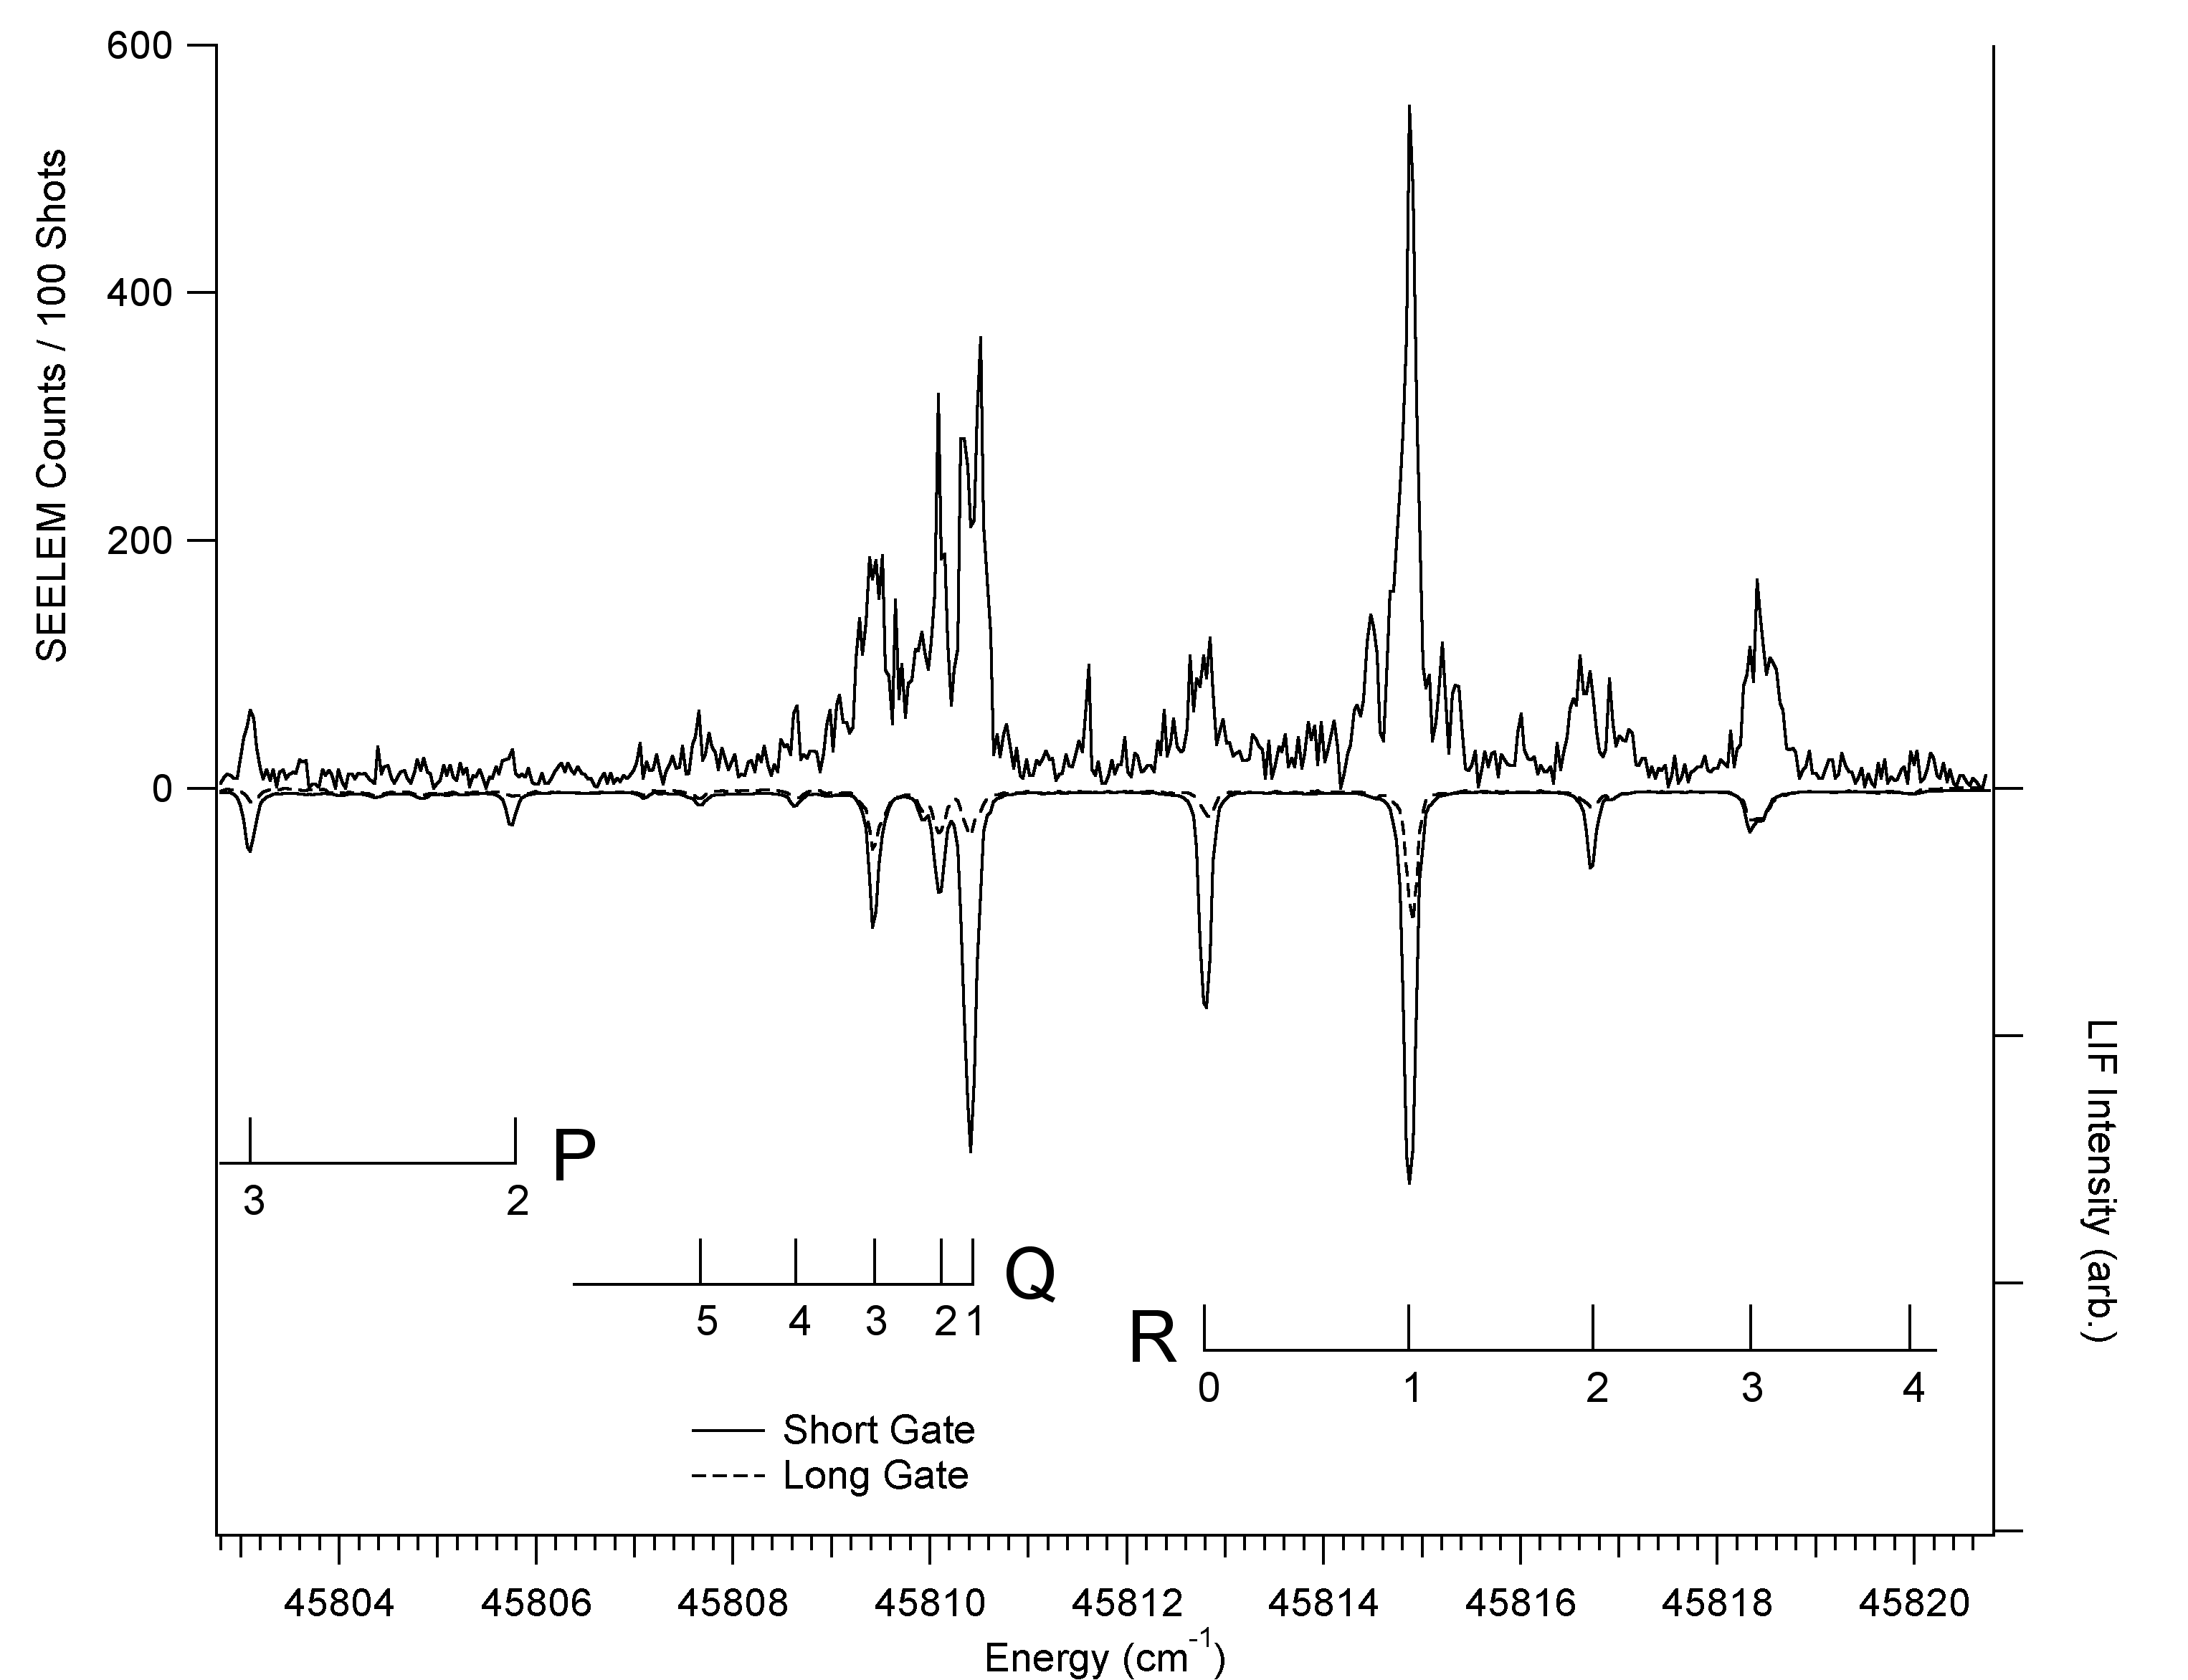
\includegraphics[width=8in,angle=90]{spectrum-32b2.png}
\end{figure}

\subsection{Analysis: LIF/SEELEM intensity distributions}

\TODO{Run 2131b2 spectra through c.o.g. analysis.}

\POINT{Make the case for center of gravity metric. Use tools from
  Chapter 2.  Refute arguments against.  (See p.109 of 4/2007--8/2007
  notebook.)}

% \POINT{Present error analysis for gated fluorescence
%   measurements. (Have an appendix for ``optimum'' gate width? Notebook
%   11/2005--3/2006)}

\POINT{Use gated fluorescence and SEELEM intensity comparison to make
  the case for weak coupling. Lifetimes tabulated in notebook
  8/2007--10/2007}

% \POINT{Lifetimes do not match intensities -- does this point to
%   complicated coupling?  (See p.99 of 8/2007--10/2007 notebook, and
%   p.31 of 4/2007--8/2007 notebook.)}

\subsection{Analysis: Unexpected band intensities resulting from
  competing Coriolis and Darling-Dennison interactions}

\TODO{Adapt analysis from paper.}  While spectra involving vibrational
excitation have been traditionally analyzed in terms of normal modes,
it is well known that at significant excitation energy, the modes can
become strongly mixed, and large deviations from the small-amplitude,
rigid-molecule normal vibrations are expected.  In the case of the
$\nu_4$ and $\nu_6$ bending vibrations of $\tilde{A}$-state acetylene,
the pure normal mode description is not adequate. Superpositions of
normal modes are required to describe the wavefunctions of levels
involving the low-frequency excited state bending vibrations.

Though no deperturbation of the $2^13^1B^2$ polyad has been attempted,
the qualitative structure of the polyad can be anticipated by drawing
parallels to the $B^2$ polyad, which has recently been analyzed by
Merer et al.  In that work, an effective, multiresonant Hamiltonian
was constructed to take into account the effects of Darling-Dennison
resonance in addition to the $a$- and $b$-axis Coriolis interactions
described by Utz and coworkers.  This effective Hamiltonian was fitted
to the available experimental data from the high-sensitivity LIF
spectra of the $B^2$ polyad (containing the $4^2$ ($a_g$), $6^2$
($a_g$), and $4^16^1$ ($b_g$) basis states) recorded in a molecular
beam. It was found that the strength of the Darling-Dennison
interaction is sufficient to cause nearly complete ($\sim$50:50)
mixing of the $4^2$ and $6^2$ basis states in the $J$=$K_a$=0
levels. In the absence of other effects, the nominal $4^2$ and $6^2$
levels would contain the same fractional contributions from the $4^2$
and $6^2$ basis states and would only differ in the phase of that
mixing.  The $4^16^1$ state remains essentially pure in $J$=$K_a$=0.

For levels with $J>0$, the Coriolis interactions must be
considered. In particular, we focus on the $K_a$=1 sublevels that, as
a consequence of the c-type selection rules for the $\tilde{A}^1A_u
\leftarrow \tilde{X} ^1\Sigma_g^+$ transition, dominate the LIF
spectrum recorded from the ground ($\ell"$=0) vibrational level. In
$K_a$=1, the 2:2 Darling-Dennison interaction strongly mixes the
near-resonant $4^2$ and $6^2$ zero-order levels, as it does in
$K_a$=0. However, in $K_a$=1, the a-axis Coriolis matrix elements now
connecting the $4^16^1$ state to the $4^2$ and $6^2$ basis states have
opposite phases. If the Darling-Dennison interaction is
prediagonalized, the phases of the Coriolis matrix elements result in
a strong interference effect. The nominal $4^2$ level has the proper
phase to mix strongly with the $4^16^1$, $b_g$ vibrational symmetry
level, whereas the nominal $6^2$ level has the wrong phase.

Extending this argument to the $2^13^1B^2$ polyad, the strongly mixed
nature of $2^13^14^2$ and $2^13^16^2$ permits $2^13^14^16^1$ to
interact with only one of the two mixed vibrational levels. An
analysis of this interference effect, which depends on the relative
phase of the anharmonic and Coriolis matrix elements, shows that the
 $2^13^14^16^1$ basis state is strongly Coriolis coupled to the nominal
$2^13^14^2$ level but not to the nominal $2^13^16^2$ level. As a result
of the interference effect, a significant amount of $b_g$ character is
mixed exclusively into $2^13^14^2$.

Although this preliminary, semi-quantitative analysis is based on a
local fit of the interactions within $B^2$, rather than a more global
model for all of the $S_1$ bending polyads of acetylene, the interactions
most pertinent to the observed SEELEM spectra can be characterized
using this simple, local model.

\POINT{Contrasting behavior of modes 4 and 6 attributed to differing
  amounts of $b_g$ vibrational character -- they are otherwise
  completely mixed.}

\POINT{Could the amount of $b_g$ character be J-dependent?}

\POINT{Alternating pattern of intensity -- does this point to a $T_3$
  level with $K=0$?}

\subsection{Discussion}

\TODO{Adapt from paper.}  Even a qualitative analysis of the SEELEM
spectra can reveal salient features of the singlet $\sim$ triplet
interaction dynamics. Despite the fact that the LIF signal in
$2^13^16^2$ is a factor of 3 larger than the LIF signal of
$2^13^14^2$, the corresponding SEELEM spectra do not share this same
intensity ratio. In stark contrast to the LIF signal, the SEELEM
signal for $2^13^16^2$ is exceedingly weak, while the $2^13^14^2$
SEELEM signal is comparatively intense. This difference in SEELEM
activity can be interpreted in terms of the strength of the
interaction between the bright $S_1$ state and a unique perturbing
vibrational level of $T_3$.

It is known that the singlet $\sim$ triplet interaction mechanism in
the $\tilde{A}^1A_u$ state of acetylene is a doorway-mediated process,
where the coupling of $S_1$ to the dark $T_{1,2}$ states is mediated
by $T_3$.  In light of the doorway model, there are two possible
explanations for the difference between the two SEELEM spectra. The
first is a vibrational overlap argument, where vibrational overlap
between the $S_1$ and $T_3$ vibrational wavefunctions promotes or
suppresses SEELEM signal. A second possibility is that the phases of
the $a$-axis Coriolis matrix elements connecting the $4^16^1$ state to
the $4^2$ and $6^2$ basis states result in an interference effect that
gives rise to a difference in how the two $S_1$ vibrational levels
interact with $T_3$.

In the normal mode model, $\nu_4$ and $\nu_6$ normal vibrations are
rigorously conserved. In a more accurate polyad model, $2^13^16^2$ and
$2^13^14^2$ belong to a strongly mixed superposition of modes, rather
than pure normal modes. Since the vibrational levels are strongly
mixed, a simple Franck-Condon argument would predict the SEELEM
spectra of $2^13^16^2$ and $2^13^14^2$ to be nearly identical.

The simplest explanation for the difference between the two observed
SEELEM spectra lies in an investigation of the Coriolis interaction
within the mixed $2^13^1B^2$ $K_a$=1 polyad. From the effective
Hamiltonian analysis, the main difference between the wavefunctions of
the two $S_1$ $2^13^1B^2$ vibrational levels probed in the experiment
is the amount of admixed $b_g$ vibrational character, taking into account
the interference between anharmonic and Coriolis interaction matrix
elements. Although $2^13^14^16^1$ is both short-lived and would
fluoresce strongly, it is not easily visible in either SEELEM or LIF
spectra due to low excitation probability and spectral overlap with
the near degenerate $1^13^1$ $K_a$=1 level. Since the a-type Coriolis
interaction causes $2^13^14^16^1$ to interact with (nominal)
$2^13^14^2$, but not with (nominal) $2^13^16^2$, a logical conclusion
is that the $b_g$ vibrational character in the nominal $2^13^14^2$ level
is what gives rise to the enhancement in SEELEM intensity. The
interaction of nominal $2^13^14^2$ with $T_3$ is due to the mixing of
$b_g$ vibrational character into nominal $2^13^14^2$.

While $a$-type Coriolis coupling gives rise to the SEELEM signal in the
region of $2^13^14^2$ $K_a$=1, $b$-type Coriolis coupling may
contribute to the $J$-dependence of the SEELEM signal near the LIF
spectrum of $2^13^16^2$ Ka=1.  The scaling of the $b$-axis Coriolis
matrix elements goes as $\sqrt{J(J+1)-K(K+1)}$ , which results in strongly
$J$-dependent mixing between basis states differing in both $K_a$ and
the vibrational quantum numbers. This strong $J$-dependence also leads
to states with anomalous effective rotational structure. Since the
higher $K_a$ sublevels of $2^13^14^16^1$ can mix with the nominal
$2^13^16^2$ $K_a$=1 level, these are likely candidates for the sources
of $b_g$ character, which is shown here to be essential to the
interaction with the nearby $T_3$ level.



% \section{Investigation of ``pure bending'' vibrational levels:
%   $4^16^3$ and $4^3$}

% \subsection{Results}

% \TODO{Figures of spectra for these bands (with assignments)}

% \POINT{SEELEM spectrum of $4^1 6^3$ is very weak (See data from Feb 2,
%   p.50 of 1/2007--3/2007 notebook.)}

% \POINT{SEELEM spectrum of $4^3$ $K=2$ hot band (Jan 16A) -- need to
%   check this in Watson's atlas.}

% \subsection{Analysis and discussion}

% \POINT{Discuss in terms of global structure of bending polyads.  (See
%   AHS and Merer's predictions on p.39 of 1/2007--3/2007 notebook.)}

% \POINT{The conclusion is that we probably don't have enough S/N with
%   these bands to perform any SEELEM/LIF intensity analysis.  Can we
%   get any amount of info from lifetimes or quantum beats?}

% \POINT{Uniformity of coupling in both Q and (P,R) branches -- does
%   this imply that $K\ne0$?}


\section{Investigation of a near-isoenergetic set of $2^n3^m$ ($n+m=3$)
  vibrational levels}

\subsection{Observations}

\TODO{Figures of spectra for these bands (with assignments). See IGOR
  task list.}

\POINT{SEELEM spectrum of $2^2 3^1$ (Oct/Nov 2006, see ``similitude''
  calculations, p.62 of Sep 2006--Jan 2007 notebook.)}



\POINT{SEELEM spectrum of $2^1 3^2$ P, Q-branch (See Jan 16A+B,
  p.124--127 of 9/2006--1/2007 notebook, also assignments on p.2 of
  1/2007--3/2007 notebook.)}  This spectrum is shown in Figure
\ref{fig:spectrum-2132}.

\begin{figure}
  \caption{
    % Simultaneously recorded LIF and SEELEM spectra of the
    % acetylene $V^2_04^2_0K^1_0$ $\tilde{A}^1A_u \leftarrow
    % \tilde{X}^1\Sigma_g$ transition.
    Simultaneously recorded surface electron ejection by laser excited
    metastables (SEELEM, upper trace) and ultraviolet laser-induced
    fluorescence (UV-LIF, lower trace) spectra of the $2^13^2$ $K_a$=1
    sublevel of the $\tilde{A}^1A_u \leftarrow \tilde{X} ^1\Sigma_g^+$
    electronic transition. A delayed, integrated fluorescence signal
    is shown as a dotted trace in the UV-LIF spectrum.}
  \label{fig:spectrum-2132}
  \centering
  \includegraphics[width=8in,angle=90]{spectrum-2132.pdf}
\end{figure}


\POINT{SEELEM spectrum of $3^3$ $K=2$ hot band (See Jan 22C, p.31,34
  of 1/2007--3/2007 notebook.)}  This spectrum is shown in Figure
\ref{fig:spectrum-33k2}.

\begin{figure}
  \caption{
    Simultaneously recorded surface electron ejection by laser excited
    metastables (SEELEM, upper trace) and ultraviolet laser-induced
    fluorescence (UV-LIF, lower trace) spectra of the $3^3$ $K_a$=2
    sublevel of the $\tilde{A}^1A_u \leftarrow \tilde{X} ^1\Sigma_g^+$
    electronic transition. A delayed, integrated fluorescence signal
    is shown as a dotted trace in the UV-LIF spectrum.}
  \label{fig:spectrum-33k2}
  \centering
  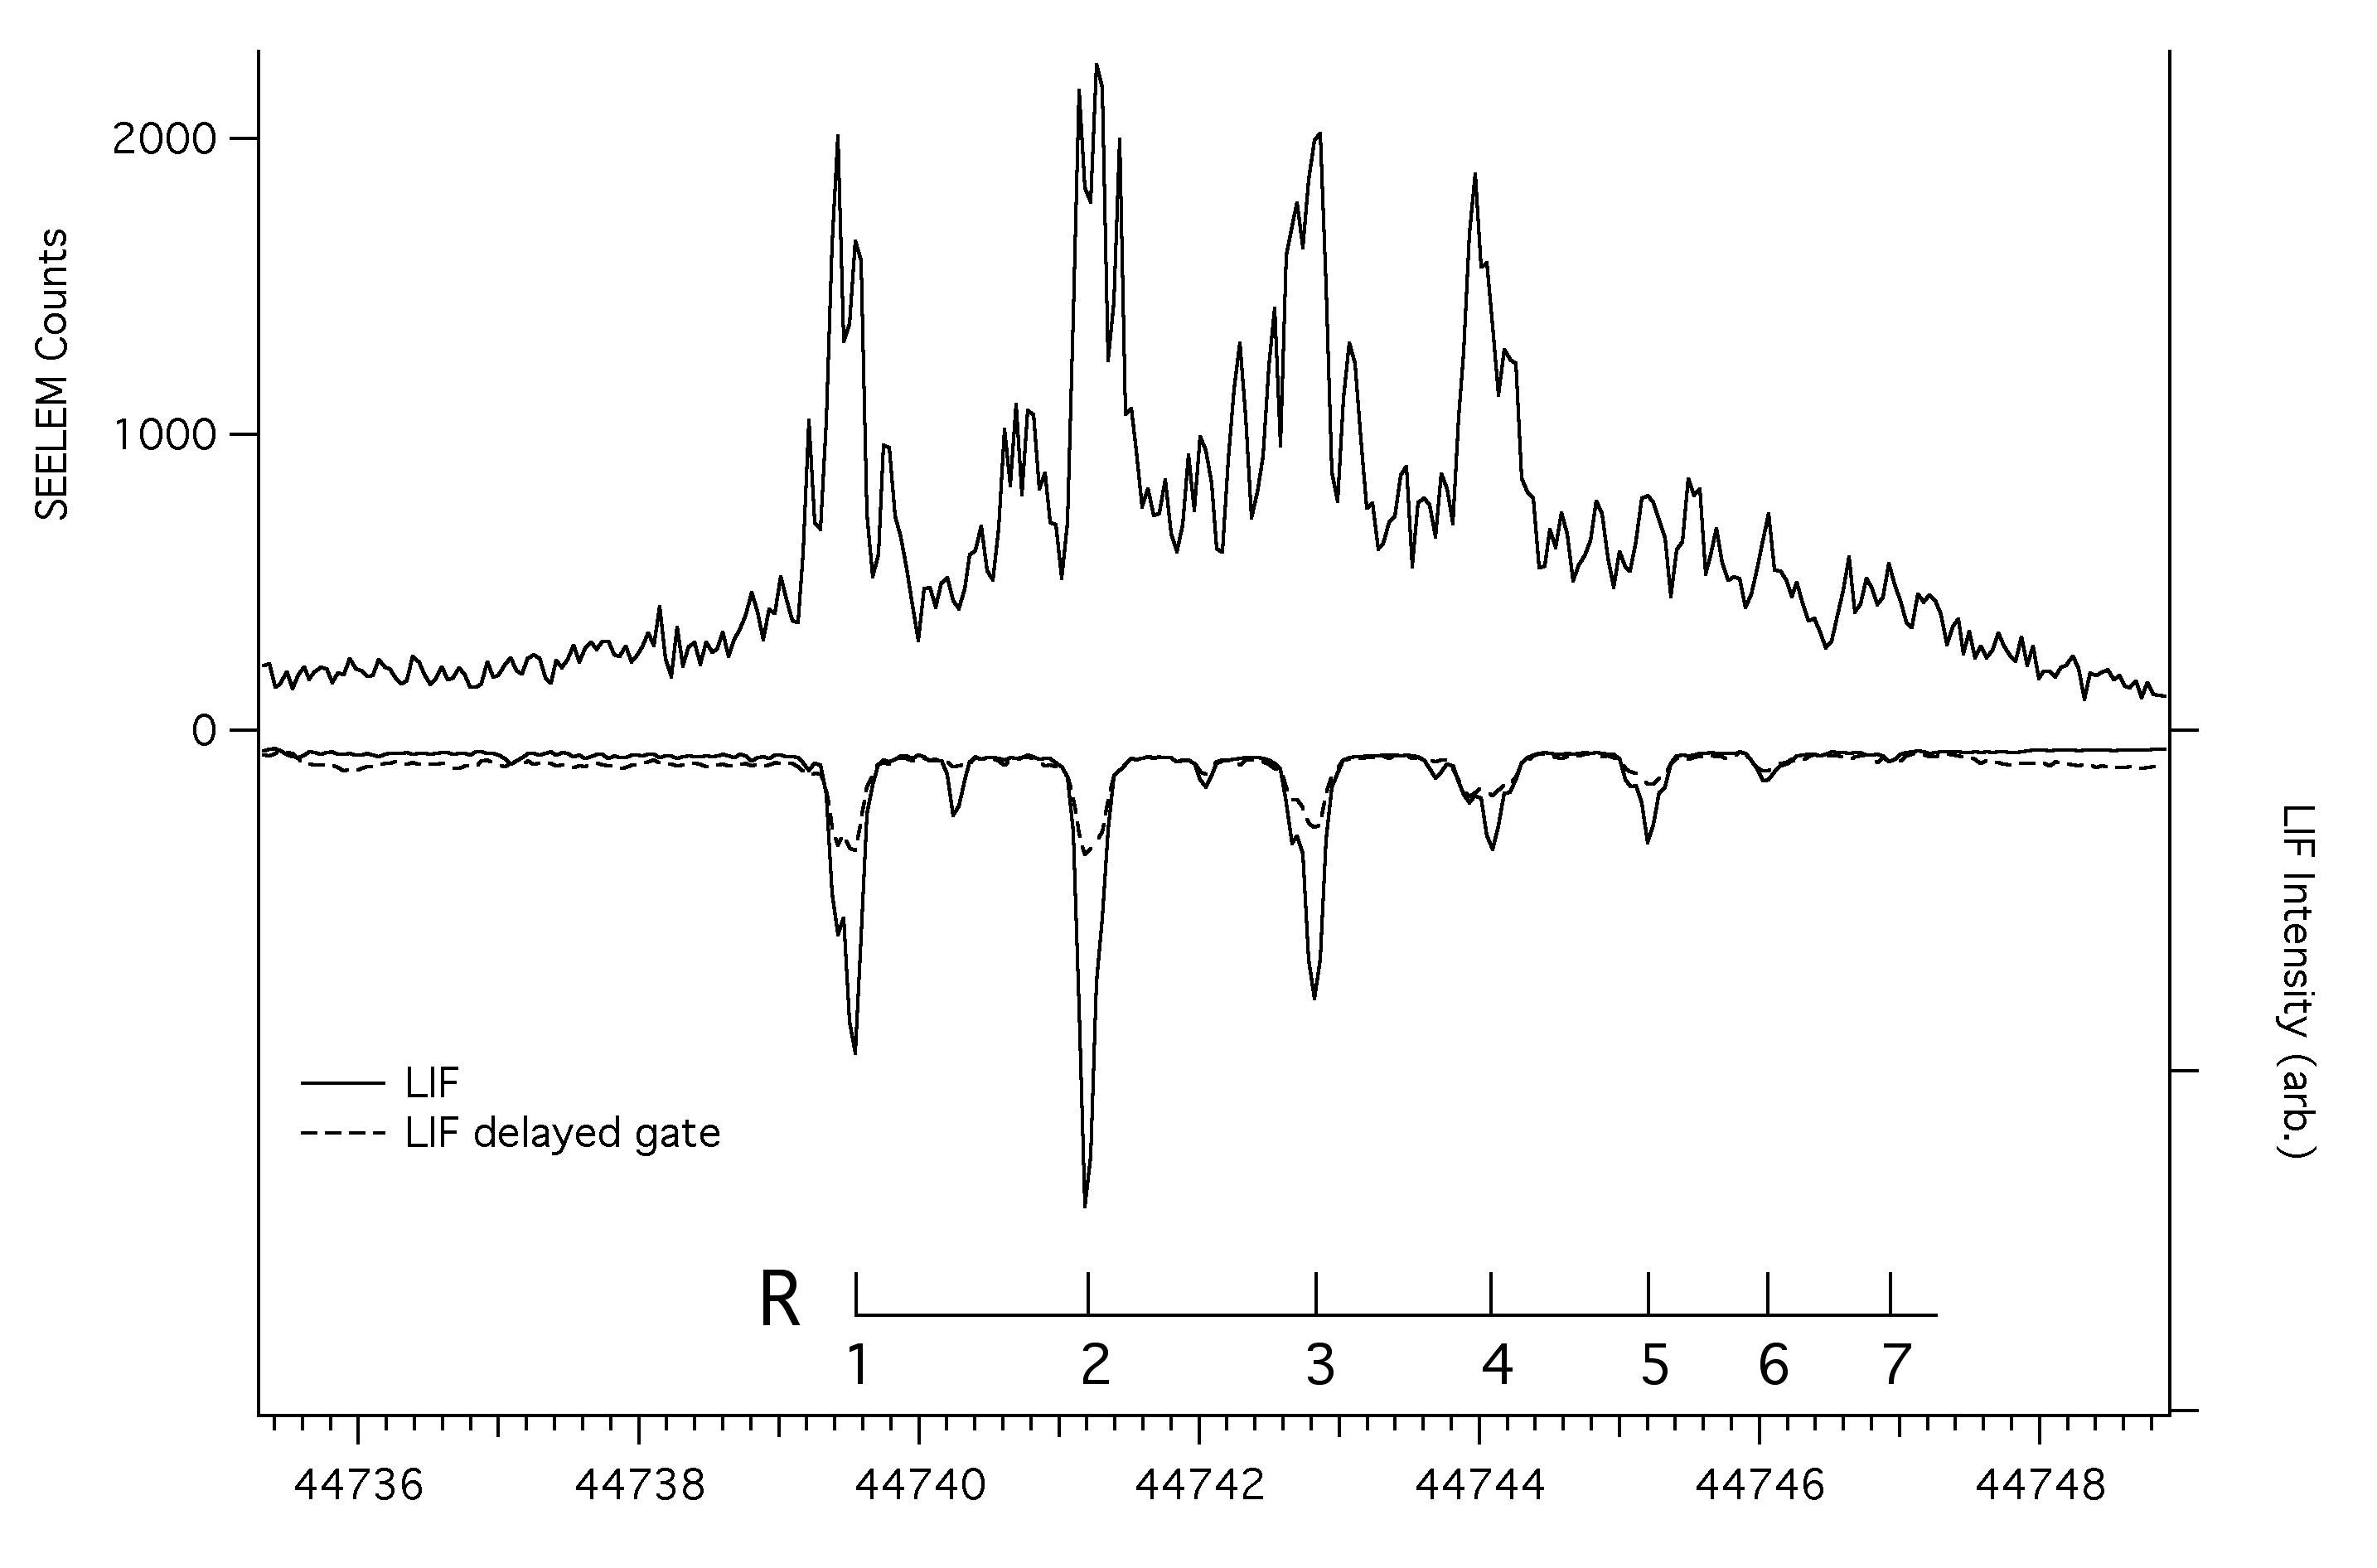
\includegraphics[width=8in,angle=90]{spectrum-33k2.png}
\end{figure}

\subsection{LIF/SEELEM intensity distributions}

\subsection{Analysis}

\POINT{Analyze the remaining bands under the assumption of distant
  doorway coupling via $T_3$.  Include center-of-gravity metrics,
  lifetime/gated fluorescence metrics, and intensity distributions.}

\section{Conclusion}

\TODO{Adapt from paper.}  SEELEM / LIF spectra of two related bands in
the $\tilde{A}^1A_u \leftarrow \tilde{X} ^1\Sigma_g^+$ system of
acetylene have been recorded in order to elucidate the nature of
S1$\sim$T3 interaction in acetylene. A simple model is proposed which
explains the intensity effects and features in the contrasting SEELEM
spectra in the region of the $2^13^16^2$ and $2^13^14^2$ vibrational
levels. The $2^13^16^2$ $K_a$=1 and $2^13^14^2$ $K_a$=1 vibrational
levels are strongly mixed by anharmonic Darling-Dennison
interactions. The major difference between these two $S_1$ vibrational
levels is the significant amount of $b_g$ vibrational character mixed
into $2^13^14^2$ by a-axis Coriolis coupling. This gives rise to
enhanced S1$\sim$T3 mixing in the nominal 213142 level, as observed.
When examined together, both the SEELEM / LIF experiment and polyad
theoretical arguments add important new details about the nature of
the doorway mediated mechanism for intersystem crossing in acetylene.

\POINT{The LIF/SEELEM spectra for the progression of $2^n3^m$ levels
  shows the expected}

\POINT{Darling-Dennison and A-type Coriolis coupling play a major role
  in determining the singlet-triplet interactions for vibrational
  levels involving modes 4 and 6 \cite{ochi91}.}

\POINT{Make the case for studying the bending motions without
  complications from Darling-Dennison or $a$-type Coriolis coupling.}

\bibliography{master}
\bibliographystyle{plain}
\end{document}